\documentclass[a4paper,10pt]{article}
\usepackage[margin=1in]{geometry}
\usepackage{amsmath,amsthm,amssymb,amsfonts,stmaryrd}
\usepackage{soul}
\usepackage{array}
\usepackage{empheq}
\usepackage{xfrac}
\usepackage{minibox}
\usepackage{enumitem}
	\setlist{nosep} % or \setlist{noitemsep} to leave space around whole list
\usepackage{color}
\usepackage{blkarray}
\setcounter{MaxMatrixCols}{20}
\usepackage{showlabels}
\usepackage{arydshln}	% Dotted lines in arrays
\usepackage{adjustbox}
\usepackage{hyperref}
\hypersetup{
  colorlinks   = true, %Colours links instead of ugly boxes
  urlcolor     = blue, %Colour for external hyperlinks
  linkcolor    = blue, %Colour of internal links
  citecolor   = red %Colour of citations
}
\usepackage{cleveref}
\usepackage{multirow}


\newtheorem{lemma}{Lemma}
\newtheorem{definition}{Definition}
\newtheorem{theorem}{Theorem}
\newtheorem{corollary}{Corollary}

\newcommand{\tcb}{\textcolor{blue}}
\newcommand{\tcr}{\textcolor{red}}
\newcommand{\todo}[1]{\textcolor{red}{[TODO\@: #1]}}


\begin{document}
\allowdisplaybreaks

% ---------------------------------------------------------------------------------------------- %
% ---------------------------------------------------------------------------------------------- %
% ---------------------------------------------------------------------------------------------- %
\section{New linear theory}

Consider a similar preconditioner as in
\Cref{sec:solve:inv}, but with some constant $\gamma \mapsto
(\gamma I - \widehat{\mathcal{L}})^{-2}$. The resulting preconditioned
operator takes the form
%
\begin{align}\nonumber
\mathcal{P}_\gamma & =
(\gamma I - \mathcal{L})^{-2}\Big[(nI - \mathcal{L})^2 + \beta^2 I\Big] \\ \nonumber
& = (\gamma I - \mathcal{L})^{-2}\Big[((\eta-\gamma)I + (\gamma I - \mathcal{L}))^2 + \beta^2 I\Big] \\
% & = (\gamma I - \mathcal{L})^{-2}\Big[(\gamma-\eta)^2I - 2(\gamma-\eta)(\gamma I - \mathcal{L}) +
% 	(\gamma I - \mathcal{L})^2 + \beta^2 I\Big] \nonumber\\
& = I - 2(\gamma-\eta)(\gamma I - \mathcal{L})^{-1} + (\beta^2 + (\gamma-\eta)^2)(\gamma I -
	\mathcal{L})^{-2} \nonumber\\
& = I - 2\frac{\gamma-\eta}{\gamma}\left(I - \tfrac{1}{\gamma}\mathcal{L}\right)^{-1} +
	\frac{\beta^2 + (\gamma-\eta)^2}{\gamma^2}
	\left(I - \tfrac{1}{\gamma}\mathcal{L}\right)^{-2}.\label{eq:prec_k}
\end{align}
%
Note that in \eqref{eq:prec_k} we have a quadratic polynomial in
$(I - \tfrac{1}{\gamma}\mathcal{L})^{-1}$. Although this provides
nice structure, the field of values analysis applied in \Cref{sec:solve:inv}
becomes much more complicated due to no necessary relation between
$\langle A\mathbf{x},\mathbf{x}\rangle$ and
$\langle A^2\mathbf{x},\mathbf{x}\rangle$ for general operators $A$. Thus, here
we take a different approach, analyzing the condition number of the preconditioned
operator, $\mathcal{P}_\gamma$, similar to as done for SPD matrices in \cite{exh}.
Although the conditioning does not yield immediate GMRES bounds as the field of values
analysis does (or as conditioning does for bounds on CG convergence), it still
provides a robust measure of the effectiveness and scalability of the
preconditioner.
Moving forward we will limit ourselves to considering $\eta \leq \gamma \leq \
\tfrac{\eta^2+\beta^2}{\eta}$, which limits to the natural case of $\gamma = \eta$
as $\beta \to 0$.

%

% %
% Under the additional assumption of $\mathcal{L}^2 \geq 0$, $\gamma = \eta$
% yields bounds
% %
% \begin{align*}
% \textnormal{cond}(\mathcal{P}_{\gamma_*}) \leq 1 + \frac{\beta^2}{\eta^2}.
% \end{align*}
% %

\begin{theorem}[Conditioning of preconditioned operator]\label{th:cond}
Suppose Assumptions \ref{ass:eig} and \ref{ass:fov} hold, that is, $\eta > 0$
and $W(\mathcal{L}) \leq 0$ \eqref{eq:fov}. Let $\mathcal{P}_\gamma$ denote
the preconditioned operator, where $((\eta + i\beta)I -
\widehat{\mathcal{L}})((\eta - i\beta)I - \widehat{\mathcal{L}})$ is
preconditioned with $(\gamma I - \widehat{\mathcal{L}})^{-2}$.
Define $\gamma_* = \sqrt{\eta^2+\beta^2}$. Then
%
\begin{align}\label{eq:gammastar}
\textnormal{cond}(\mathcal{P}_{\gamma_*}) \leq 
	3\sqrt{1+\frac{\beta^2}{\eta^2}} - 2.
\end{align}

Assume additionally that $W(\mathcal{L}^2) \geq 0$. Then for
$\eta \leq \gamma \leq \gamma_*$ 
\begin{align}\label{eq:cond_gen}
\textnormal{cond}(\mathcal{P}_\gamma) \leq \frac{\gamma}{\eta}
	\left(1 + \frac{\beta^2 + (\gamma-\eta)^2}{\gamma^2}\right).
\end{align}
\end{theorem}
\begin{proof}
Recall for matrix $A$, cond$(A) = \|A\|\|A^{-1}\|$.
First, consider bounding $\|\mathcal{P}_\gamma\|$ for $\gamma \geq \eta$:
%
\begin{align}\nonumber
\|\mathcal{P}_\gamma\| & = \left\| I - 2\frac{\gamma-\eta}
	{\gamma}\left(I - \tfrac{1}{\gamma}\mathcal{L}\right)^{-1} +
		\frac{\beta^2 + (\gamma-\eta)^2}{\gamma^2}
		\left(I - \tfrac{1}{\gamma}\mathcal{L}\right)^{-2} \right\| \\
% & \leq \left\| I - 2\frac{\gamma-\eta}
% 	{\gamma}\left(I - \tfrac{1}{\gamma}\mathcal{L}\right)^{-1}\right\| +
% 		\frac{\beta^2 + (\gamma-\eta)^2}{\gamma^2}\left\|
% 		\left(I - \tfrac{1}{\gamma}\mathcal{L}\right)^{-2} \right\| \\
& \leq \left\| I - 2\frac{\gamma-\eta}
	{\gamma}\left(I - \tfrac{1}{\gamma}\mathcal{L}\right)^{-1}\right\| +
		\frac{\beta^2 + (\gamma-\eta)^2}{\gamma^2}\left\|
		\left(I - \tfrac{1}{\gamma}\mathcal{L}\right)^{-1} \right\|^2 \nonumber \\
& \leq \left\| I - 2\frac{\gamma-\eta}
	{\gamma}\left(I - \tfrac{1}{\gamma}\mathcal{L}\right)^{-1}\right\| +
		\frac{\beta^2 + (\gamma-\eta)^2}{\gamma^2}. \label{eq:P0}
\end{align}
%
For the first term, note that maximizing over $\mathbf{v}\in\mathbb{R}^n$ and
letting $\mathbf{v} := (I - \tfrac{1}{\gamma}\mathcal{L})\mathbf{w}$,
%
\begin{align*}
\left\| I - 2\tfrac{\gamma-\eta}
	{\gamma}(I - \tfrac{1}{\gamma}\mathcal{L})^{-1}\right\|^2
		& = \sup_{\mathbf{v}\neq\mathbf{0}} \frac{\left\| [I - 2\frac{\gamma-\eta}
	{\gamma}(I - \tfrac{1}{\gamma}\mathcal{L})^{-1}]\mathbf{v}\right\|^2}{\|\mathbf{v}\|^2} 
= \sup_{\mathbf{w}\neq\mathbf{0}} \frac{\left\| (I - \tfrac{1}{\gamma}\mathcal{L} -
		2\frac{\gamma-\eta}{\gamma}I )\mathbf{w}\right\|^2}{\|(I - \tfrac{1}{\gamma}\mathcal{L})
		\mathbf{w}\|^2} \\
% & = \sup_{\mathbf{w}\neq\mathbf{0}} \frac{\left\|[(1 - 2\frac{\gamma-\eta}{\gamma})
% 	I - \tfrac{1}{\gamma}\mathcal{L}]\mathbf{w}\right\|^2}{\|(I - \tfrac{1}{\gamma}\mathcal{L})
% 		\mathbf{w}\|^2} \\
&\hspace{-5ex} = \sup_{\mathbf{w}\neq\mathbf{0}} \frac{|1 - 2\tfrac{\gamma-\eta}{\gamma}|^2\|\mathbf{w}\|^2
	- \tfrac{1}{\gamma}(1 - 2\tfrac{\gamma-\eta}{\gamma})\langle (\mathcal{L} + \mathcal{L}^T)
		\mathbf{w},\mathbf{w}\rangle + \tfrac{1}{\gamma}^2\|\mathcal{L}\mathbf{w}\|^2}
	{\|\mathbf{w}\|^2 - \tfrac{1}{\gamma}\langle (\mathcal{L} + \mathcal{L}^T)
		\mathbf{w},\mathbf{w}\rangle + \tfrac{1}{\gamma}^2\|\mathcal{L}\mathbf{w}\|^2}.
\end{align*}
%
Note that by assumption, $\gamma \geq \eta$, which implies
$0 \leq 2\tfrac{\gamma-\eta}{\gamma}  < 2$, and 
$|1 - 2\tfrac{\gamma-\eta}{\gamma}| < 1$. In addition, we assume $W(\mathcal{L})\leq 0$,
which implies $\langle (\mathcal{L}+\mathcal{L}^T)\mathbf{w},\mathbf{w}\rangle \leq 0$
(see \Cref{th:fov}), and
$2\tfrac{\gamma-\eta}{\gamma^2} \geq 0$, which implies the term
$2\tfrac{\gamma-\eta}{\gamma^2}\langle (\mathcal{L}+\mathcal{L}^T)
	\mathbf{w},\mathbf{w}\rangle\leq 0$. Appealing to these two inequalities,
%
\begin{align} \label{eq:P1}
\left\| I - 2\tfrac{\gamma-\eta}
	{\gamma}(I - \tfrac{1}{\gamma}\mathcal{L})^{-1}\right\|^2
& < \sup_{\mathbf{w}\neq\mathbf{0}} \frac{\|\mathbf{w}\|^2
	- \tfrac{1}{\gamma}\langle (\mathcal{L} + \mathcal{L}^T)
		\mathbf{w},\mathbf{w}\rangle + \tfrac{1}{\gamma}^2\|\mathcal{L}\mathbf{w}\|^2}
	{\|\mathbf{w}\|^2 - \tfrac{1}{\gamma}\langle (\mathcal{L} + \mathcal{L}^T)
		\mathbf{w},\mathbf{w}\rangle + \tfrac{1}{\gamma}^2\|\mathcal{L}\mathbf{w}\|^2} 
= 1.
\end{align}
%
Combining \eqref{eq:P0} and \eqref{eq:P1} yields
%
\begin{align}\label{eq:Pgamma}
\|\mathcal{P}_\gamma\| \leq 1 + \frac{\beta^2 + (\gamma-\eta)^2}{\gamma^2}.
\end{align}

Now consider bounding $\|\mathcal{P}_\gamma^{-1}\|$ from above. Let $s_{\max}(A)$
and $s_{\min}(A)$ denote the maximum and minimum singular value of matrix $A$,
respectively, and recall
%
\begin{align*}
\|\mathcal{P}_\gamma^{-1}\| = s_{\max}(\mathcal{P}_\gamma^{-1})
	& = \frac{1}{s_{\min}(\mathcal{P}_\gamma)}, \hspace{5ex}\textnormal{where}\hspace{2ex}
s_{\min}(\mathcal{P}_\gamma) =
	\min_{\mathbf{v}\neq\mathbf{0}} \frac{\|\mathcal{P}_\gamma\mathbf{v}\|}{\|\mathbf{v}\|}.
\end{align*}
%
Thus, consider the minimum singular value of $P_\gamma$. Letting $\mathbf{v} :=
(I - \tfrac{1}{\gamma}\mathcal{L})^{2}\mathbf{w}$,
%
\begin{align}\nonumber
s_{\min}(\mathcal{P}_\gamma)^2 & = \min_{\mathbf{v}\neq\mathbf{0}}
	\frac{\left\| \left[I - 2\frac{\gamma-\eta}{\gamma}(I - \tfrac{1}{\gamma}
		\mathcal{L})^{-1} + \frac{\beta^2 + (\gamma-\eta)^2}{\gamma^2}
		(I - \tfrac{1}{\gamma}\mathcal{L})^{-2}\right]\mathbf{v} \right\|^2}
	{\|\mathbf{v}\|^2} \\
& = \min_{\mathbf{v}\neq\mathbf{0}}
	\frac{\left\| \left[(I - \tfrac{1}{\gamma}\mathcal{L})^{2} - 2\frac{\gamma-\eta}{\gamma}
		(I - \tfrac{1}{\gamma} \mathcal{L}) + \frac{\beta^2 + (\gamma-\eta)^2}{\gamma^2} I
		\right]\mathbf{w} \right\|^2}
	{\|(I - \tfrac{1}{\gamma}\mathcal{L})^{2}\mathbf{w}\|^2} \nonumber\\
& = \min_{\mathbf{v}\neq\mathbf{0}}
	\frac{\left\| \left[(I - \tfrac{1}{\gamma}\mathcal{L})^{2} + 
		\tfrac{\eta^2+\beta^2-\gamma^2}{\gamma^2} I + 2\frac{\gamma-\eta}{\gamma^2}
		\mathcal{L}) \right]\mathbf{w} \right\|^2}
	{\|(I - \tfrac{1}{\gamma}\mathcal{L})^{2}\mathbf{w}\|^2}.\label{eq:smin0}
\end{align}
%

For ease of notation, define
%
\begin{align*}
c_I & := \tfrac{\eta^2+\beta^2-\gamma^2}{\gamma^2} , \hspace{5ex}
c_{\mathcal{L}} := 2\frac{\gamma-\eta}{\gamma^2},
\end{align*}
%
noting that for $\eta\leq\gamma\leq\sqrt{\eta^2+\beta^2}$, $c_I,c_{\mathcal{L}} \geq 0$.
Now, collect like terms in \eqref{eq:smin0} and expand the norm to yield
%
\begin{align}\label{eq:smin_ex}
\begin{split}
& s_{\min}(\mathcal{P}_\gamma)^2 \\
& = \min_{\mathbf{w}\neq\mathbf{0}}
	\frac{\left\| \left[(1+c_I)I - (\tfrac{2}{\gamma}-c_{\mathcal{L}})\mathcal{L} +
		\tfrac{1}{\gamma^2}\mathcal{L}^2\right]\mathbf{w} \right\|^2}
	{\left\|\left(I - \tfrac{2}{\gamma}\mathcal{L} +
		\tfrac{1}{\gamma^2}\mathcal{L}^2\right)\mathbf{w} \right\|^2} \\
& =  \min_{\mathbf{w}\neq\mathbf{0}}
	\frac{\|(1+c_I)\mathbf{w}+\tfrac{1}{\gamma^2}\mathcal{L}^2\mathbf{w}\|^2 +
		(\tfrac{2}{\gamma}-c_{\mathcal{L}})^2\|\mathcal{L}\mathbf{w}\|^2 -
		2(1+c_I)(\tfrac{2}{\gamma}-c_{\mathcal{L}})\langle\mathcal{L}\mathbf{w},\mathbf{w}\rangle -
		2\tfrac{2-\gamma c_{\mathcal{L}}}{\gamma^3}\langle\mathcal{L}(\mathcal{L}\mathbf{w}),
			\mathcal{L}\mathbf{w}\rangle}
	{\|\mathbf{w}+\tfrac{1}{\gamma^2}\mathcal{L}^2\mathbf{w}\|^2 +
		\tfrac{4}{\gamma^2}\|\mathcal{L}\mathbf{w}\|^2 -
		\tfrac{4}{\gamma}\langle\mathcal{L}\mathbf{w},\mathbf{w}\rangle -
		\tfrac{4}{\gamma^3}\langle\mathcal{L}(\mathcal{L}\mathbf{w}),\mathcal{L}\mathbf{w}\rangle}.
\end{split}
\end{align}
%
By assumption on $W(\mathcal{L})\leq 0$ and $\eta\leq\gamma\leq\sqrt{\eta^2+\beta^2}$,
all terms in the numerator and denominator are non-negative (note, $\mathbf{w}$ and
$\tfrac{1}{\gamma^2}\mathcal{L}^2\mathbf{w}$ were kept together in norm to avoid
the difficulties that arise in analyzing $\langle\mathcal{L}^2\mathbf{w},\mathbf{w}\rangle$).
For numerator $\mathcal{N}$ and denominator $\mathcal{D}$, if $\widehat{K}\mathcal{N}
\geq \mathcal{D}$, then $\mathcal{N}/\mathcal{D} \geq 1 / \widehat{K}$. For 
$\|\mathcal{L}\mathbf{w}\|^2$, $\langle\mathcal{L}\mathbf{w},\mathbf{w}\rangle$,
and $\langle\mathcal{L}(\mathcal{L}\mathbf{w}),\mathcal{L}\mathbf{w}\rangle$,
we can directly bound the ratio of constants in the numerator and denominator.
For $\|\mathcal{L}\mathbf{w}\|^2$, we have
%
\begin{align*}
\widehat{K}(\tfrac{2}{\gamma}-c_{\mathcal{L}})^2 \geq \frac{4}{\gamma^2}
	\hspace{5ex}\Longleftrightarrow\hspace{5ex}
\widehat{K} \geq \frac{\gamma^2}{\eta^2},
\end{align*}
%
while $\langle\mathcal{L}\mathbf{w},\mathbf{w}\rangle$ requires
%
\begin{align*}
2\widehat{K}(1+c_I)(\tfrac{2}{\gamma}-c_{\mathcal{L}})\geq \frac{4}{\gamma},
	\hspace{5ex}\Longleftrightarrow\hspace{5ex}
\widehat{K} \geq \frac{\gamma^3}{\eta(\eta^2+\beta^2)},
\end{align*}
%
and $\langle\mathcal{L}(\mathcal{L}\mathbf{w}),\mathcal{L}\mathbf{w}\rangle$
requires
%
\begin{align*}
2\widehat{K}\tfrac{2-\gamma c_{\mathcal{L}}}{\gamma^3} \leq \frac{4}{\gamma^3},
	\hspace{5ex}\Longleftrightarrow\hspace{5ex}
\widehat{K} \geq \frac{\gamma}{\eta}.
\end{align*}
%
Because we want a lower bound on $\mathcal{N}/\mathcal{D} \geq 1/\widehat{K}$,
we seek the maximum required $\widehat{K}$ of the above ratios. For
$\gamma \in[\eta,\sqrt{\eta^2+\beta^2}]$, the maximum of the
above ratios ends up being $\widehat{K} := \tfrac{\gamma^2}{\eta^2}$.

The difficult ratio to bound in \eqref{eq:smin_ex} ends up being 
$\|(1+c_I)\mathbf{w}+\tfrac{1}{\gamma^2}\mathcal{L}^2\mathbf{w}\|^2$ and the
similar denominator term, $\|\mathbf{w}+\tfrac{1}{\gamma^2}\mathcal{L}^2\mathbf{w}\|^2$.
Here we consider two cases:\\
\\
%%%%%
\underline{$\boldsymbol{\gamma_* = \sqrt{\eta^2+\beta^2}}$}: Under this specific choice, we
get the nice cancellation that $c_I = 0$, and have matching terms
$\|\mathbf{w}+\tfrac{1}{\gamma^2}\mathcal{L}^2\mathbf{w}\|^2$ in the numerator
and denominator of \eqref{eq:smin_ex}. Then, the maximum ratio of numerator 
to denominator terms is $\widehat{K} := \tfrac{\gamma^2}{\eta^2}$ derived above,
and we can bound $\|P_{\gamma}^{-1}\|$ via
%
\begin{align}\label{eq:gammas_bound}
\|P_{\gamma}^{-1}\| & = \frac{1}{s_{\min}(P_{\gamma}^{-1})} 
	\leq \frac{1}{1/\sqrt{\widehat{K}}} 
	= \frac{\sqrt{\eta^2+\beta^2}}{\eta} =
	\sqrt{1+\frac{\beta^2}{\eta^2}}.
\end{align}
%
Combining with \eqref{eq:Pgamma} for $\gamma = \gamma_*$ and simplifying
completes the proof of \eqref{eq:gammastar}.\\
\\
%%%%%
\noindent
\underline{\textbf{Nonnegative $\mathcal{L}^2$}}: Suppose $W(\mathcal{L}^2) \geq 0$.
Given we are minimizing over real vectors, we can write $\langle\mathcal{L}^2\mathbf{w},
\mathbf{w} \rangle := \cos(\theta)\|\mathcal{L}^2\mathbf{w}\|\|\mathbf{w}\|$ for some
angle $\theta$. By assumption $W(\mathcal{L}^2) \geq 0$, we have $\cos(\theta)\geq 0$.
Taking the ratio of these individual terms then yields
%
\begin{align}\label{eq:problem}
\frac{\|(1+c_I)\mathbf{w}+\tfrac{1}{\gamma^2}\mathcal{L}^2\mathbf{w}\|^2}
	{\|\mathbf{w}+\tfrac{1}{\gamma^2}\mathcal{L}^2\mathbf{w}\|^2}
& = \frac{(1+c_I)^2\|\mathbf{w}\|^2+\tfrac{1}{\gamma^4}\|\mathcal{L}^2\mathbf{w}\|^2
	+ 2\cos(\theta)(1+c_I)\|\mathcal{L}^2\mathbf{w}\|\|\mathbf{w}\|}
	{\|\mathbf{w}\|^2+\tfrac{1}{\gamma^4}\|\mathcal{L}^2\mathbf{w}\|^2
	+ 2\cos(\theta)\|\mathcal{L}^2\mathbf{w}\|\|\mathbf{w}\|}.
\end{align}
%
Letting $x := \tfrac{\|\mathcal{L}\mathbf{w}\|}{\|\mathbf{w}\|}$, we can
cancel $1/\|\mathbf{w}\|^2$ from the numerator and denominator and
write \eqref{eq:problem} as a ratio of quadratic functions in $x \geq 0$:
%
\begin{align}\label{eq:x_simp}
\frac{x^2 + 2\cos(\theta)(1+c_I)x + (1+c_I)^2}{x^2 + 2\cos(\theta)x + 1}.
\end{align}
%
For $c_I\geq 0$ (corresponding to $\gamma \leq\sqrt{\eta^2+\beta^2}$)
and $\cos(\theta)\geq 0$, \eqref{eq:x_simp} is $\geq 1$ for all $x$.
%
%---------------- Comment on \gamma > \sqrt(\eta^2+\beta^2) ----------------
% It is
% also clear in \eqref{eq:x_simp} why choosing $\gamma > \sqrt{\eta^2+\beta^2}
% \implies c_I < 0$ does not appear to be advantageous, at least for this term,
% as the ratio in \eqref{eq:x_simp} is then $<1$ for all $x\geq 0$, which
% requires a larger $\widehat{K}$ and, thus, smaller bound on
% $s_{\min}(\mathcal{P}_\gamma)$.
Similar to the proof for $\gamma = \gamma_*$, the ratio in \eqref{eq:problem}
is always $\geq 1$, and the maximum required $\widehat{K}$ to bound
$\widehat{K}\mathcal{N} \geq \mathcal{D}$ for each matching term is
given by $\widehat{K} = \tfrac{\gamma^2}{\eta^2}$. Altogether,
this yields
%
\begin{align*}
\|P_{\gamma}^{-1}\| & = \frac{1}{s_{\min}(P_{\gamma}^{-1})} 
	\leq \frac{1}{1/\sqrt{\widehat{K}}} 
	= \frac{\gamma}{\eta}.
\end{align*}
%
Combining with \eqref{eq:Pgamma} completes the proof of \eqref{eq:cond_gen}.
\end{proof}
%


% % ---------------------------------------------------------------------------------------------- %
% \subsubsection{$\gamma = \sqrt{\eta^2+\beta^2}$}

% Consider the choice of $\gamma = \gamma_* = \sqrt{\eta^2+\beta^2}$. Recall $\gamma_*$
% is optimal when $\mathcal{L}$ is SPD with spectrum $\subset[0,\infty)$. It turns out,
% $\gamma_*$ provides a unique simplification here as well. From \eqref{eq:smin0}, we have
% %
% \begin{align*}
% s_{\min}(\mathcal{P}_{\gamma_*})^2 & = \min_{\mathbf{w}\neq\mathbf{0}}
% 	\frac{\left\| \left[(I - \tfrac{1}{\gamma_*}\mathcal{L})^{2} + 
% 		2\frac{\gamma_*-\eta}{\gamma_*^2} \mathcal{L}) \right]\mathbf{w} \right\|^2}
% 	{\|(I - \tfrac{1}{\gamma_*}\mathcal{L})^{2}\mathbf{w}\|^2} \\
% & = \min_{\mathbf{w}\neq\mathbf{0}}
% 	\frac{\| (I - \tfrac{1}{\gamma_*}\mathcal{L})^{2}\mathbf{w}\|^2 + 
% 		4(\frac{\gamma_*-\eta}{\gamma_*^2})^2\|\mathcal{L}\mathbf{w} \|^2 +
% 	4\frac{\gamma_*-\eta}{\gamma_*^2}\left\langle (I - \tfrac{2}{\gamma_*}\mathcal{L}+
% 		\tfrac{1}{\gamma_*^2}\mathcal{L}^2)\mathbf{w}, \mathcal{L}\mathbf{w}\right\rangle}
% 	{\|(I - \tfrac{1}{\gamma_*}\mathcal{L})^{2}\mathbf{w}\|^2} \\
% & = \min_{\mathbf{w}\neq\mathbf{0}} 1 +
% 	\frac{\left(4(\frac{\gamma_*-\eta}{\gamma_*^2})^2 - 8\frac{\gamma_*-\eta}{\gamma_*^3}\right)
% 		\|\mathcal{L}\mathbf{w} \|^2 +
% 	4\frac{\gamma_*-\eta}{\gamma_*^2}\langle\mathcal{L}\mathbf{w},\mathbf{w}\rangle 
% 	+ 4\frac{\gamma_*-\eta}{\gamma_*^4}\langle\mathcal{L}(\mathcal{L}\mathbf{w}),
% 		\mathcal{L}\mathbf{w}\rangle}
% 	{\|\mathbf{w}\|^2 + \tfrac{4}{\gamma_*^2}\|\mathcal{L}\mathbf{w}\|^2 +
% 		\frac{1}{\gamma_*^4}\|\mathcal{L}^2\mathbf{w}\|^2 - 
% 		\tfrac{4}{\gamma_*}\langle\mathcal{L}\mathbf{w},\mathbf{w}\rangle +
% 		\tfrac{2}{\gamma_*^2}\langle\mathcal{L}^2\mathbf{w},\mathbf{w}\rangle -
% 		\tfrac{4}{\gamma_*^3}\langle\mathcal{L}(\mathcal{L}\mathbf{w}),\mathcal{L}\mathbf{w}\rangle}\\
% & = \min_{\mathbf{w}\neq\mathbf{0}} 1 -
% 	\frac{\left(8\frac{\gamma_*-\eta}{\gamma_*^3} - 4(\frac{\gamma_*-\eta}{\gamma_*^2})^2\right)
% 		\|\mathcal{L}\mathbf{w} \|^2
% 	- 4\frac{\gamma_*-\eta}{\gamma_*^2}\langle\mathcal{L}\mathbf{w},\mathbf{w}\rangle 
% 	- 4\frac{\gamma_*-\eta}{\gamma_*^4}\langle\mathcal{L}(\mathcal{L}\mathbf{w}),
% 		\mathcal{L}\mathbf{w}\rangle}
% 	{\|\mathbf{w}+\tfrac{1}{\gamma_*^2}\mathcal{L}^2\mathbf{w}\|^2 +
% 		\tfrac{4}{\gamma_*^2}\|\mathcal{L}\mathbf{w}\|^2 -
% 		\tfrac{4}{\gamma_*}\langle\mathcal{L}\mathbf{w},\mathbf{w}\rangle -
% 		\tfrac{4}{\gamma_*^3}\langle\mathcal{L}(\mathcal{L}\mathbf{w}),\mathcal{L}\mathbf{w}\rangle}\\
% & \geq 1 - \max_{\mathbf{w}\not\in\textnormal{ker}(\mathcal{L})}
% 	\frac{\left(8\frac{\gamma_*-\eta}{\gamma_*^3} - 4(\frac{\gamma_*-\eta}{\gamma_*^2})^2\right)
% 		\|\mathcal{L}\mathbf{w} \|^2
% 	- 4\frac{\gamma_*-\eta}{\gamma_*^2}\langle\mathcal{L}\mathbf{w},\mathbf{w}\rangle 
% 	- 4\frac{\gamma_*-\eta}{\gamma_*^4}\langle\mathcal{L}(\mathcal{L}\mathbf{w}),
% 		\mathcal{L}\mathbf{w}\rangle}
% 	{\tfrac{4}{\gamma_*^2}\|\mathcal{L}\mathbf{w}\|^2 -
% 		\tfrac{4}{\gamma_*}\langle\mathcal{L}\mathbf{w},\mathbf{w}\rangle -
% 		\tfrac{4}{\gamma_*^3}\langle\mathcal{L}(\mathcal{L}\mathbf{w}),\mathcal{L}\mathbf{w}\rangle},
% \end{align*}
% %
% where in the last step we note that if $\mathcal{L}\mathbf{w} = \mathbf{0}$, the only
% nonzero term is $\|\mathbf{w}+\tfrac{1}{\gamma_*^2}\mathcal{L}^2\mathbf{w}\|^2 = \|\mathbf{w}\|^2$
% in the denominator, which yields one for the full equation.

% Now note that all of the terms in the numerator and denominator are non-negative,
% and we can bound the maximum from above by ensuring the leading numerator and
% denominator constants, say $c_n$ and $c_d$, satisfy $c_n/c_d \leq K$. For
% $\|\mathcal{L}\mathbf{w}\|^2$, we require
% %
% \begin{align}\nonumber
% \left(8\frac{\gamma_*-\eta}{\gamma_*^3} - 4\Big(\frac{\gamma_*-\eta}{\gamma_*^2}\Big)^2\right)
% 	& \leq \frac{4}{\gamma_*^2}K, \\
% \Longleftrightarrow\hspace{5ex}
% \left(2\frac{\gamma_*-\eta}{\gamma_*} - \Big(\frac{\gamma_*-\eta}{\gamma_*}\Big)^2\right)
% 	& \leq K
% 	\hspace{5ex}\Longleftrightarrow\hspace{5ex}
% 1 - \frac{\eta^2}{\gamma_*^2}\leq K.\label{eq:Kproof}
% \end{align}
% %
% Similarly, $\langle\mathcal{L}\mathbf{w},\mathbf{w}\rangle $ requires
% %
% \begin{align}
% 4\frac{\gamma_*-\eta}{\gamma_*^2} & \leq \frac{4}{\gamma_*}K
% 	\hspace{5ex}\Longleftrightarrow\hspace{5ex}
% 	1 - \frac{\eta}{\gamma_*} \leq K, \label{eq:Kproof2}
% \end{align}
% %
% and $\langle\mathcal{L}(\mathcal{L}\mathbf{w}),\mathcal{L}\mathbf{w}\rangle $ requires
% %
% \begin{align*}
% 4\frac{\gamma_*-\eta}{\gamma_*^4} & \leq \frac{4}{\gamma_*^3}K
% 	\hspace{5ex}\Longleftrightarrow\hspace{5ex}
% 	1 - \frac{\eta}{\gamma_*} \leq K.
% \end{align*}
% %

% Because $\gamma_* >\eta$, the largest $K$ is in \eqref{eq:Kproof}, where we define
% $K = \frac{\beta^2}{\eta^2+\beta^2} = 1 - \tfrac{\eta^2}{\gamma_*^2} >
% 1 - \tfrac{\eta}{\gamma}$. Altogether, this yields
% $s_{\min}(P_{\gamma_*}^{-1})^2 \geq 1 - K$, and
% %
% \begin{align*}
% \|P_{\gamma_*}^{-1}\| & = \frac{1}{s_{\min}(P_{\gamma_*}^{-1})} 
% 	\leq \frac{1}{\sqrt{1 - K}} 
% 	= \sqrt{1 + \frac{\beta^2}{\eta^2}}.
% \end{align*}
% %

% It is worth noting that in practice, $\|P_{\gamma_*}^{-1}\|$ is likely
% smaller and more independent of $\eta$ and $\beta$.

% ---------------------------------------------------------------------------------------------- %
% ---------------------------------------------------------------------------------------------- %
% ---------------------------------------------------------------------------------------------- %
\section{Eigenvalue analysis}

Consider preconditioning
%
\begin{align*}
\mathcal{Q}_\eta := (\eta I - \mathcal{L})^2 + \beta^2 I,
\end{align*}
%
with a preconditioner $(\gamma I - \mathcal{L})^{-2}$ for some $\gamma \geq \eta$. 
The preconditioned operator takes the form
%
\begin{align}\label{eq:gamma1}
(\gamma I- {\mathcal{L}})^{-2}\mathcal{Q}_\eta & =
	I - 2\frac{\gamma - \eta}{\gamma} ( I- \tfrac{1}{\gamma}{\mathcal{L}})^{-1} + 
	\frac{\beta^2 + (\gamma - \eta)^2}{\gamma^2}( I- \tfrac{1}{\gamma}{\mathcal{L}})^{-2}.
\end{align}
%
Suppose ${\mathcal{L}}$ is symmetric negative definite and, thus, has an orthogonal
basis of eigenvectors, and consider the conditioning of \eqref{eq:gamma1}. Assume that the
eigenvalues of $( I- \tfrac{1}{\gamma}{\mathcal{L}})^{-1} \subset (0,1)$, and are
somewhat dense in this interval. This is to be expected for parabolic problems, where the
eigenvalues of $-{\mathcal{L}}$ range from $\sim \delta t$ to $\sim \delta t/h^2$,
which typically corresponds to $\sim(0,\infty)$ as $h,\delta t\to 0$.

Note that \eqref{eq:gamma1} is a quadratic polynomial in an SPD operator, and the
eigenvalues of \eqref{eq:gamma1} are then a quadratic function $P(\lambda)$ of the
eigenvalues $\{\lambda\}$ of ${\mathcal{L}}$, where
%
\begin{align}\label{eq:quadratic2}
P(\lambda,\gamma) &:= \frac{\beta^2 + (\gamma-\eta)^2}{\gamma^2}\lambda^2 -
	2\frac{\gamma - \eta}{\gamma}\lambda + 1.
\end{align}
%
Assume that we choose $\gamma$ such that \eqref{eq:gamma1} is also SPD (choosing otherwise
would be a poor choice in terms of conditioning). Then the condition number of
\eqref{eq:gamma1} is given by
%
\begin{align}\label{eq:cond2_0}
\textnormal{cond}\left((\gamma I- {\mathcal{L}})^{-1}\mathcal{Q}_\eta\right) & =
	\frac{\lambda_{\max}\left((\gamma I- {\mathcal{L}})^{-1}\mathcal{Q}_\eta\right)}
		{\lambda_{\min}\left((\gamma I- {\mathcal{L}})^{-1}\mathcal{Q}_\eta\right)}.
\end{align}
%
Again assuming that eigenvalues $\lambda\in\sigma\left({\mathcal{L}}\right)$ take
on values $\lambda\in(0,1)$, the condition number \eqref{eq:cond0} can be expressed
precisely as $h,\delta t\to 0$ via
%
\begin{align}\label{eq:cond2_1}
\textnormal{cond}\left((\gamma I- {\mathcal{L}})^{-1}\mathcal{Q}_\eta\right) & =
	\frac{\max_{x\in(0,1)} P(x,\gamma)}{\min_{y\in(0,1)} P(y,\gamma)}.
\end{align}
%
With this closed form, it is natural to pose a minimization problem to find the
optimal $\gamma$ in terms of minimizing the condition number \eqref{eq:cond2_0}.
We make the assumption that $\eta \leq \gamma \leq \eta^2+\beta^2$, and consider
the problem
%
\begin{align*}
\gamma_\times & = \textnormal{argmin}_{\gamma \geq \eta}
	\frac{\max_{x\in(0,1)} P(x,\gamma)}{\min_{y\in(0,1)} P(y,\gamma)}.
\end{align*}
%

Note that $P(\lambda)$ \eqref{eq:quadratic2} is a quadratic polynomial in $\lambda$,
and thus its maximum over a closer interval $[0,1]$ will be obtained at one of the
endpoints,
%
\begin{align*}
P(0,\gamma) = 1, \hspace{3ex} P(1,\gamma) = \frac{\eta^2+\beta^2}{\gamma^2}.
\end{align*}
%
For the maximum eigenvalue, this yields
%
\begin{align}\label{eq:max0}
\lambda_{\max} & = \begin{cases} 
	\frac{\eta^2+\beta^2}{\gamma^2} & \gamma < \sqrt{\eta^2+\beta^2}, \\
	1 & \gamma \geq \sqrt{\eta^2+\beta^2}.
	\end{cases}
\end{align}
%

The minimum eigenvalue will either be obtained at a critical point, or if there is
no critical point in the interval $(0,1)$, at the other endpoint than the maximum
was obtained at. To consider the critical point, we differentiate \eqref{eq:quadratic2}
and obtain the root
%
\begin{align}\label{eq:lambda_0}
\lambda_0 &:= \frac{\gamma(\gamma-\eta)}{\beta^2+(\gamma-\eta)^2}.
\end{align}
%
For $\gamma \geq \eta$, $\lambda_0 \geq 0$. To consider when $\lambda_0\leq 1$, we can
set it equal to one and rearrange for the equivalent condition
%
\begin{align}\label{eq:ass1}
\gamma \leq \frac{\beta^2+\eta^2}{\eta}.
\end{align}
%
Assuming \eqref{eq:ass1} holds, we have $\lambda_0 \in[0,1]$, and
the minimum value of $P(\lambda,\gamma)$ in $\lambda$ is achieved at $\lambda_0$,
%
\begin{align}\label{eq:min0}
\lambda_{\min} & = \frac{\beta^2}{\beta^2 + (\gamma-\eta)^2}.
\end{align}
%

Combining \eqref{eq:max0}, \eqref{eq:ass1}, and \eqref{eq:min0} yields
%
\begin{align}\label{eq:cases0}
\textnormal{cond}\left((\gamma I- {\mathcal{L}})^{-1}\mathcal{Q}_\eta\right) & =
\begin{cases} 
	\frac{(\eta^2+\beta^2)(\beta^2 + (\gamma-\eta)^2)}
		{\beta^2\gamma^2}
		& \eta \leq \gamma < \sqrt{\eta^2+\beta^2}, \\
	\frac{\beta^2 + (\gamma-\eta)^2}{\beta^2}
		& \sqrt{\eta^2+\beta^2} \leq \gamma \leq \frac{\eta^2+\beta^2}{\eta}.
	\end{cases}
\end{align}
%
Here we have ended up at the result from The 2017 paper in (3.22) and (3.23),
and they say both of the above equations are minimized at the interface
%
\begin{align}\label{eq:gamma_opt0}
\gamma_\times := \sqrt{\eta^2+\beta^2}.
\end{align}
%

% ---------------------------------------------------------------------------------------------- %
% ---------------------------------------------------------------------------------------------- %
% ---------------------------------------------------------------------------------------------- %
\section{Nonlinear/Schur complement}

In the nonlinear setting we need to solve
%
\begin{align}\label{eq:block}
\begin{bmatrix} \eta I - \widehat{\mathcal{L}} & \phi I\\
	-\frac{\beta^2}{\phi} I & \eta I - \widehat{\mathcal{L}}\end{bmatrix},
\end{align}
%
with Schur complement of \eqref{eq:block} given by
%
\begin{align}\label{eq:simpSchur}
S & := \eta I - \widehat{\mathcal{L}} + \beta^2 (\eta I - \widehat{\mathcal{L}})^{-1}.
\end{align}
%
The initial idea is to consider a block lower triangular preconditioner for \eqref{eq:block},
given by
%
\begin{equation}\label{eq:Lprec}
L_P := \begin{bmatrix} \eta I - \widehat{\mathcal{L}} & \mathbf{0} \\ -\frac{\beta^2}{\phi} I
	& \widehat{S}\end{bmatrix}^{-1}.
\end{equation}
%
This raises the natural question as to how do we approximate $S^{-1}?$ An easy first
choice is to let $\widehat{S} := \eta I - \widehat{\mathcal{L}}$. Then the FOV analysis
from the linear case immediately applies, and we know it is robust. Such an approach has
the additional benefit of only requiring one preconditioner for both stages \tcb{[OAK: This is true only for the simplified Newton case though; in the quasi-Newton algorithm, diagonal blocks in the $2 \times 2$ operator are different, so they don't use the same preconditioner anyway.]}. Unfortunately,
tests have also shown this choice to be suboptimal as the number of stages gets large,
that is, convergence gets slower for higher order.

% ---------------------------------------------------------------------------------------------- %
% ---------------------------------------------------------------------------------------------- %
\subsection{A factorization}

In the linear setting, we were actually solving the equation
%
\begin{align*}
(\eta I - \widehat{\mathcal{L}})^2 + \beta^2 I,
\end{align*}
%
which we found to be better (and scalably) preconditioned by $(k I - \widehat{\mathcal{L}})^{-2}$,
for $k = \sqrt{\eta^2+\beta^2}$. How do we handle this with the Schur complement? One
option is to factor $S$,
%
\begin{align*}
S & := \Big((\eta I - \widehat{\mathcal{L}})^2 + \beta^2I\Big)(\eta I - \widehat{\mathcal{L}})^{-1}, \\
\mapsto\hspace{5ex}
S^{-1} & = (\eta I - \widehat{\mathcal{L}})\Big((\eta I - \widehat{\mathcal{L}})^2 + \beta^2I\Big)^{-1},
\end{align*}
%
where we can then precondition the inverse term in $S^{-1}$ exactly as we did in the
linear setting. The downside here is we have introduced an additional solve, because
now we must apply preconditioning to the (1,1)-block, followed by \textit{two}
preconditioning iterations to the Schur complement, as well as an additional matvec.
That being said, for some of the linear advection-diffusion problems, the modified
constant led to convergence $3-4\times$ faster, so it is possible this additional
step of preconditioning is worth it. 

Similarly, we can also suck the extra inverse out and solve it separately. Writing
out the block LDU inverse of \eqref{eq:block} we have
%
\begin{align}\label{eq:ldu}
\begin{bmatrix} \eta I - \widehat{\mathcal{L}} & \phi I\\
	-\frac{\beta^2}{\phi} I & \eta I - \widehat{\mathcal{L}}\end{bmatrix}^{-1}
= \begin{bmatrix} I & -\phi(\eta I - \widehat{\mathcal{L}})^{-1} \\ \mathbf{0} & I\end{bmatrix}
	\begin{bmatrix} (\eta I - \widehat{\mathcal{L}})^{-1} & \mathbf{0} \\ \mathbf{0} & S^{-1} \end{bmatrix}
	\begin{bmatrix} I & \mathbf{0} \\ \tfrac{\beta^2}{\phi}(\eta I - \widehat{\mathcal{L}})^{-1} & I
	\end{bmatrix}.
\end{align}
%
In practice it is typically not advantageous to directly apply an LDU inverse,
because when solving the Schur-complement inverse in an iterative fashion, each
application of $S$ requires computing an exact inverse of the (1,1)-block. However,
with some algebra, we can rewrite \eqref{eq:ldu} as
%
\begin{align}\label{eq:ldu2}
\begin{bmatrix} \eta I - \widehat{\mathcal{L}} & \phi I\\
	-\frac{\beta^2}{\phi} I & \eta I - \widehat{\mathcal{L}}\end{bmatrix}^{-1}
= \begin{bmatrix} (\eta I - \widehat{\mathcal{L}})^{-1} & \mathbf{0} \\ \mathbf{0} & I\end{bmatrix}
\begin{bmatrix} I & -\phi I \\ \mathbf{0} & I\end{bmatrix}
	\begin{bmatrix} I & \mathbf{0} \\ \mathbf{0} &
		\Big((\eta I - \widehat{\mathcal{L}})^2 + \beta^2I\Big)^{-1} \end{bmatrix}
	\begin{bmatrix} I & \mathbf{0} \\ \tfrac{\beta^2}{\phi} I & \eta I - \widehat{\mathcal{L}}
	\end{bmatrix}.
\end{align}
%
Here we have introduced an additional mat-vec by $\eta I - \widehat{\mathcal{L}}$,
and otherwise separated the inverse into two separate pieces, $(\eta I - \widehat{\mathcal{L}})^{-1}$,
which is a standard backward Euler step, and
$\Big((\eta I - \widehat{\mathcal{L}})^2 + \beta^2I\Big)^{-1}$, which is exactly the
problem we solved in the linear setting, which we would precondition with two
applications of $(k I - \widehat{\mathcal{L}})^{-1}$, for $k=\sqrt{\eta^2+\beta^2}$.
The nice thing about this problem and formulation is that although 

% ---------------------------------------------------------------------------------------------- %
% ---------------------------------------------------------------------------------------------- %
\subsection{A modified $\gamma$: the SPD case}

Suppose $-\mathcal{L}$ is SPSD with a spectrum $\subset [0,\infty)$, and
consider preconditioning $S$ with $(\gamma I- \widehat{\mathcal{L}})^{-1}$ for
some $\gamma \neq \eta$. The preconditioned operator then takes the form
%
\begin{align}\nonumber
(\gamma I- \widehat{\mathcal{L}})^{-1}S & = (\gamma I - \widehat{\mathcal{L}})^{-1}
	\left[ (\gamma I - \widehat{\mathcal{L}}) + (\eta-\gamma)I + \beta^2 (\eta I - \widehat{\mathcal{L}})^{-1}\right] \\
& = I - (\gamma - \eta)( \gamma I- \widehat{\mathcal{L}})^{-1} + 
	\beta^2( \gamma I- \widehat{\mathcal{L}})^{-1}
		( \eta I-\widehat{\mathcal{L}})^{-1} \nonumber\\
& = I - \frac{\gamma - \eta}{\gamma} ( I- \tfrac{1}{\gamma}\widehat{\mathcal{L}})^{-1} + 
	\frac{\beta^2}{\gamma\eta}( I- \tfrac{1}{\gamma}\widehat{\mathcal{L}})^{-1}
		( I- \tfrac{1}{\eta}\widehat{\mathcal{L}})^{-1},\label{eq:gamma0}
\end{align}
%
with spectrum given by
%
\begin{align}\label{eq:eig_gamma}
\mathcal{F}(\gamma,\lambda) :&= 
	1 - \frac{\gamma-\eta}{\gamma + \lambda} + \frac{\beta^2}{(\gamma + \lambda)(\eta+\lambda)},
\end{align}
%
where $\lambda\in\sigma(-\mathcal{L})$. If we choose $\gamma>\eta$,
\eqref{eq:gamma0} is SPD, \tcb{(BS: above is not necessarily SPD for $0<\gamma<\eta$.
Often it would be, but you can pick $\eta>0,\lambda,\beta\geq 0$ such that
it is not)} and the condition number of \eqref{eq:gamma0} is given by
%
\begin{align}\label{eq:cond0}
\textnormal{cond}\left((\gamma I- \widehat{\mathcal{L}})^{-1}S\right) & =
	\frac{\lambda_{\max}\left((\gamma I- \widehat{\mathcal{L}})^{-1}S\right)}
		{\lambda_{\min}\left((\gamma I- \widehat{\mathcal{L}})^{-1}S\right)}.
\end{align}
\tcr{[OK: 
I'm a bit confused by the SPD thing; am I making a mistake in the following derivation? We want to show for which range of $\gamma$ ${\cal F} > 0$ (which implies the operator is positive definite). Have 
\begin{align*}
\mathcal{F}(\gamma,\lambda) := 
	1 - \frac{\gamma-\eta}{\gamma + \lambda} + \frac{\beta^2}{(\gamma + \lambda)(\eta+\lambda)} 
	=
1 + \frac{(\eta - \gamma) (\eta + \lambda) + \beta^2}{(\gamma + \lambda) (\eta + \lambda)}. 
\end{align*}
So, if $(\gamma + \lambda) (\eta + \lambda) > 0$, which is always true if we assume $\gamma > 0$, since $\eta > 0$ and $\lambda \geq 0$, then:
\begin{align*}
{\cal F} > 0 
&\Longrightarrow 
(\eta - \gamma) (\eta + \lambda) + (\gamma + \lambda) (\eta + \lambda) + \beta^2  > 0 \\
&\Longrightarrow 
[\eta - \gamma + \gamma + \lambda] (\eta + \lambda) + \beta^2  > 0 \\
& \Longleftrightarrow (\eta + \lambda)^2 + \beta^2 > 0.
\end{align*}
This last statement is always true, and the only assumption we made in arriving here is $\gamma > 0$. Therefore ${\cal F} > 0$ and the operator is positive definite?
]}

%
As $h,\delta t\to 0$, it is typical for parabolic problems that
the spectrum $\lambda\in\sigma\left(-\widehat{\mathcal{L}}\right)$
becomes increasingly dense in the interval $[0,\infty)$. For such limiting
behavior, the condition number \eqref{eq:cond0} can be expressed
precisely as
%
\begin{align}\label{eq:cond1}
\textnormal{cond}\left((\gamma I- \widehat{\mathcal{L}})^{-1}S\right) & \mapsto
	\frac{\max_{\lambda\in[0,\infty)} \mathcal{F}(\gamma,\lambda)}
		{\min_{\lambda\in[0,\infty)} \mathcal{F}(\gamma,\lambda)}.
\end{align}
%

With this closed form, it is natural to pose a minimization problem to find the
optimal $\gamma$ in terms of minimizing the condition number \eqref{eq:cond0}.
Let $\gamma > \eta$ and consider the problem
%
\begin{align}\label{eq:gam_opt}
\gamma_* & = \textnormal{argmin}_{\gamma>\eta}
	\frac{\max_{\lambda\in[0,\infty)} \mathcal{F}(\gamma,\lambda)}
		{\min_{\lambda\in[0,\infty)} \mathcal{F}(\gamma,\lambda)}.
\end{align}
%
Minima and maxima in $\lambda$ may be obtained at one of the endpoints,
$\lambda = 0$ or $\lambda\to\infty$, or at a critical point of \eqref{eq:eig_gamma}
in $\lambda$. Taking the partial with respect to $\lambda$, we have
%
\begin{align}\label{eq:partial_l}
\frac{\partial\mathcal{F}}{\partial\lambda} & =
	\frac{(\gamma-\eta)(\eta+\lambda)^2 - \beta^2(\gamma+\eta+2\lambda)}
		{(\gamma+\lambda)^2(\eta+\lambda)^2}.
\end{align}
%
Noting that the denominator is nonnegative for $\eta,\gamma>0$ and $\lambda \geq 0$,
the critical points are obtained at zeros of the numerator in \eqref{eq:partial_l},
which can be written as a quadratic polynomial in $\lambda$:
%
\begin{align*}
(\gamma-\eta)\lambda^2 - 2(\eta^2+\beta^2 - \eta\gamma)\lambda + 
	\gamma(\eta^2-\beta^2) - \eta(\eta^2+\beta^2) = 0.
\end{align*}
%
Working through the algebra, for $\gamma \neq \eta$ the two real roots are given by
%
\begin{align}\label{eq:roots}
\lambda_{\pm} & := \frac{\beta^2 + \eta^2 - \gamma\eta \pm
	\beta\sqrt{\beta^2 + (\gamma-\eta)^2}}{\gamma-\eta}.
\end{align}
%
Thus, we have four potential points at which a maximum or minimum in $\lambda$
can be achieved, $\{0,\infty, \lambda_\pm\}$. Working through the algebra yields
%
\begin{align}\label{eq:F_gamma}
\begin{split}
\mathcal{F}(\gamma,\infty) & = 1, \hspace{20ex}
\mathcal{F}(\gamma,\lambda_+) = \frac{2\beta}{\beta + \sqrt{\beta^2 + (\gamma-\eta)^2}}, \\
\mathcal{F}(\gamma,0) & = 1 + \frac{\eta^2+\beta^2-\eta\gamma}{\eta\gamma},
\hspace{4ex}
\mathcal{F}(\gamma,\lambda_-) = \frac{2\beta}{\beta - \sqrt{\beta^2 + (\gamma-\eta)^2}}.
\end{split}
\end{align}
%

Note that $\mathcal{F}(\gamma,\lambda_-) < 0$, which contradicts the previously
stated result that $\mathcal{F}(\gamma,\lambda)$ is SPD for $\gamma > \eta$
and $\lambda\geq 0$, implying $\lambda_- < 0$.
Thus we are left with three critical points to consider, 
$\{0,\lambda_+,\infty\}$. Further, observe that
%
\begin{align*}
\mathcal{F}(\gamma,\lambda_+) = \frac{2\beta}{\beta + \sqrt{\beta^2 + (\gamma-\eta)^2}}
	= \frac{2}{1 + \sqrt{1 + (\gamma-\eta)^2/\beta^2}} < 1 = \mathcal{F}(\gamma,\infty),
\end{align*}
%
for all $\gamma > \eta$, with equality for $\gamma = \eta$.
It follows that the maximum of ${\cal F}(\gamma,\lambda)$ w.r.t.
$\lambda$ must thus occur for $\lambda \in \{ 0, \infty \}$. Evaluating
\eqref{eq:F_gamma}, we have
%
\begin{align*}
\max_{\lambda\in[0,\infty)} \mathcal{F}(\gamma,\lambda) & = 
\begin{cases}
\displaystyle
\mathcal{F}(\gamma,0) 
= 
\frac{1}{\gamma} \left(\eta + \frac{\beta^2}{\eta} \right), 
\quad 
& \eta < \gamma \leq \eta +  \tfrac{\beta^2}{\eta}, \\
\displaystyle
\mathcal{F}(\gamma,\infty) 
= 
1, \quad & \eta + \tfrac{\beta^2}{\eta} \leq \gamma < \infty
\end{cases}.
\end{align*}
%

For the minimum, because $\mathcal{F}(\gamma,\lambda_+) < \mathcal{F}(\gamma,\infty),
\forall \gamma > \eta$, the minimum cannot occur for $\lambda \to \infty$, which
implies the minimum of ${\cal F}(\gamma,\lambda)$ w.r.t. $\lambda$ must occur
at $\lambda \in \{0, \lambda_+\}$. For $\gamma \geq \eta + \beta^2 / \eta$,
${\cal F}(\gamma, \lambda_+) < 1 \leq {\cal F}(\gamma, 0)$. To consider
$\eta < \gamma < \eta + \beta^2 / \eta$, define
%
\begin{align*}
{\cal G}(\gamma) = \mathcal{F}(\gamma,0) -  \mathcal{F}(\gamma,\lambda_+),
	\quad \eta < \gamma \leq \eta + \beta^2 / \eta.
\end{align*}
%
To determine which value of ${\lambda} \in \{0, \lambda_+ \}$ minimizes
${\cal F}(\gamma, \lambda)$ we can consider the sign of ${\cal G}$. From
above, we know that ${\cal G} > 0$ for $\gamma = \eta + \beta^2/\eta$, so
we seek roots $\hat{\gamma}\in(\eta,\eta+\beta^2/\eta]$, such that
${\cal G}(\hat{\gamma}) = 0$, indicating a sign change in ${\cal G}$.

\tcb{(BS: next two equations not obvious, is first one relevant?)} \tcr{[OK: First equation was kind of relevant. I rewrote what was below to make clearer where these things come from. Let me know if still unclear.]}

Setting ${\cal G}(\hat{\gamma}) = 0$ and assuming $\beta > 0$, we have
\begin{align*}
\frac{2\beta}{\beta + \sqrt{\beta^2 + (\hat{\gamma}-\eta)^2}} 
=
\frac{1}{\hat{\gamma}} \left(\eta + \frac{\beta^2}{\eta} \right) 
\quad \Longrightarrow \quad
2\beta \eta \hat{\gamma} -\beta(\eta^2 + \beta^2) 
= 
\beta(\eta^2 + \beta^2) \sqrt{\beta^2 + (\hat{\gamma}-\eta)^2}. 
\end{align*}
Squaring both sides of the latter equation leads to a quadratic equation in $\hat{\gamma}$, which we will denote $z(\hat{\gamma}) = 0$. However, note that the RHS of the latter equation is positive, and so for any root of $z$ to also be a root of ${\cal G}$, it must satisfy $\hat{\gamma} > \tfrac{1}{2} \big( \eta + \beta^2 / \eta)$. Carrying out the calculation, we have
\begin{align*}
z(\hat{\gamma}) = \big[ 4 \beta^2 \eta^2 - (\eta^2 + \beta^2)^2 \big] \hat{\gamma}^2 + 2 \eta (\eta^2 + \beta^2)(\eta^2 - \beta^2) \hat{\gamma} - \eta^2(\eta^2 + \beta^2)^2.
\end{align*}
%
Note that the discriminant of $z(\hat{\gamma})$ is zero, implying
$z(\hat{\gamma})$ has one real root. This root is
%
\begin{align} \label{eq:gamma_hat}
\hat{\gamma} = \eta \frac{\eta^2 + \beta^2}{\eta^2 - \beta^2}. 
\end{align}
%
If $\eta < \beta$, then $\hat{\gamma} < 0$ which violates the necessary condition that $\hat{\gamma} > \tfrac{1}{2} \big( \eta + \beta^2 / \eta)$ for $\hat{\gamma}$ to also be a root of ${\cal G}$. For $\eta > \beta$, it is straightforward to show that
$\hat{\gamma} > \eta+\beta^2/\eta$, and, so, this root of ${\cal G}$ does not lie in the interval $(\eta,\eta+\beta^2/\eta]$. Thus, ${\cal G}$ has no sign changes
in the interval $(\eta,\eta+\beta^2/\eta]$, implying
${\cal F} (\gamma, \lambda_+) < {\cal F}(\gamma, 0)$ for $\eta < \gamma
\leq \eta + \beta^2/\eta.$ Combining with the earlier discussion, we have
%
\begin{align*}
\min_{\lambda\in[0,\infty)} \mathcal{F}(\gamma,\lambda) &=
	\mathcal{F}(\gamma,\lambda_+) =
\frac{2\beta}{\beta + \sqrt{\beta^2 + (\gamma-\eta)^2}}
	\quad \eta < \gamma < \infty.
\end{align*}
%

Altogether, the condition number \eqref{eq:cond1} is given by the continuous function of $\gamma>\eta$
\begin{align}
\label{eq:condc}
c(\gamma) 
\coloneqq
\textnormal{cond}\left((\gamma I- \widehat{\mathcal{L}})^{-1}S\right)  
=
\begin{cases}
\displaystyle
\frac{1}{\gamma} \left(\eta + \tfrac{\beta^2}{\eta} \right) \frac{\beta + \sqrt{\beta^2 + (\gamma-\eta)^2}}{2\beta}
\eqqcolon c_1(\gamma), 
\quad & \eta < \gamma \leq \eta + \tfrac{\beta^2}{\eta},
\\[3ex]
\displaystyle
\frac{\beta + \sqrt{\beta^2 + (\gamma-\eta)^2}}{2\beta}
\eqqcolon c_2(\gamma), 
\quad &\eta + \tfrac{\beta^2}{\eta} \leq \gamma < \infty 
\end{cases}.
\end{align}
Now, we want to find the minimizer $\gamma_*$ of the condition number $c$
as defined in \eqref{eq:gam_opt}.
First, note that $c_2$ is an increasing function over the interval for
which it is defined. Thus, its minimum is achieved at the left boundary
of its domain, $\textnormal{argmin}_{(\eta + \beta^2/\eta) \leq \gamma
< \infty} c_2(\gamma) = \eta + \beta^2/\eta$, with minimum value
%
\begin{align} 
\label{eq:c2_min}
c_2\left(\eta + \frac{\beta^2}{\eta} \right) = \frac{1}{2} \left( 1 + \sqrt{1 + \left( \frac{\beta}{\eta} \right)^2} \right).
\end{align}
%
For $c_1$, differentiating and solving for the roots of its derivative
yields the two critical points, $\gamma = \eta$ and $\gamma = \hat{\gamma}$
as in \eqref{eq:gamma_hat}. Neither $\eta,\hat{\gamma}\not\in(\eta, \eta + \beta^2/\eta]$,
and thus the minimum of $c_2$ will be obtained at one of the endpoints. 
By continuity of $c(\gamma)$, $c_1(\eta + \beta^2/\eta) = c_2(\eta + \beta^2/\eta)$,
given in \eqref{eq:c2_min}. Taking the limit $\lim_{\gamma\to\eta} c_1(\gamma)
= 1+\tfrac{\beta^2}{\eta^2} > c_1(\eta + \beta^2/\eta)$.

Thus, the condition number as a function of $\gamma$ \eqref{eq:condc} is
minimized at $\gamma = \eta + \beta^2 / \eta$ independent of $\beta$ and $\eta$,
where
%
\begin{align}
\gamma_* 
:= 
\underset{0 < \gamma < \infty}{\textnormal{argmin}} \; \textnormal{cond} \left((\gamma I- \widehat{\mathcal{L}})^{-1}S\right) 
= 
\eta + \frac{\beta^2}{\eta},
\end{align}
and
\begin{align} \label{eq:cond_min}
\textnormal{cond}\left((\gamma_* I- \widehat{\mathcal{L}})^{-1}S\right)
=
\frac{1}{2} \left( 1 + \sqrt{1 + \left( \frac{\beta}{\eta} \right)^2} \right).
\end{align}

While condition number \eqref{eq:cond_min} is not bounded w.r.t. $\beta/\eta$, it is very small in practice as shown in Table \ref{tab:cond}, where for the schemes we consider it's always less than 2. For example, the condition number is less than 2 for $(\beta/\eta)^2 < 8$. See also Figure \ref{fig:conds} for a comparison of the condition number using $\gamma_*$ vs. $\eta$. Also, a numerical example is shown in Table \ref{tab:cond_iters} showing a reduction in the number of iterations using $\gamma_*$ vs. $\eta$.
{
\renewcommand{\tabcolsep}{4pt}
\renewcommand{\arraystretch}{1.15}
\begin{table}[!ht]
  \centering
  \begin{tabular}{| c | c | c | cc | cc | ccc |}  % chktex 44
  \hline
Method & Stages & 2 & \multicolumn{2}{c}{3} & \multicolumn{2}{|c}{4} & \multicolumn{3}{|c|}{5} \\\hline\hline
\multirow{ 3}{*}{Gauss}
&$\beta^2/\eta^2$ & 0.33 & 0 & 0.91 & 1.59 & 0.09 & 0 & 2.36 & 0.27 \\
&$\textnormal{cond}\big((\gamma_* I- \widehat{\mathcal{L}})^{-1}S\big)$ & 1.077 & -- & 1.191 & 1.305 & 1.022 & -- & 1.43 & 1.064\\
&$\textnormal{cond}\big((\eta I- \widehat{\mathcal{L}})^{-1}S\big)$ & 1.330 & -- & 1.910 & 2.590 & 1.090 & -- & 3.460 & 1.270\\\hline
\multirow{ 3}{*}{Radau IIA}
&$\beta^2/\eta^2$ & 0.50 & 0 & 1.29 & 2.21 & 0.11 & 0 & 3.20 & 0.32	\\
&$\textnormal{cond}\big((\gamma_* I- \widehat{\mathcal{L}})^{-1}S\big)$ & 1.112 & -- & 1.257 & 1.396 & 1.027 & -- & 1.525 & 1.075\\
&$\textnormal{cond}\big((\eta I- \widehat{\mathcal{L}})^{-1}S\big)$ & 1.500 & -- & 2.290 & 3.210 & 1.110 & -- & 4.200 & 1.320\\\hline
\multirow{ 3}{*}{Lobatto IIIC}
&$\beta^2/\eta^2$ & 1 & 0 & 2.21 & 3.51 & 0.13 & 0 & 4.88 & 0.38 \\
&$\textnormal{cond}\big((\gamma_* I- \widehat{\mathcal{L}})^{-1}S\big)$ & 1.207 & -- & 1.396 & 1.562 & 1.032 & -- & 1.712 & 1.087\\
&$\textnormal{cond}\big((\eta* I- \widehat{\mathcal{L}})^{-1}S\big)$ & 2.000 & -- & 3.210 & 4.510 & 1.130 & -- & 5.880 & 1.380\\
  \hline
  \end{tabular}
  \caption{$\beta^2/\eta^2$, values of the optimal condition number $\textnormal{cond}\big((\gamma_* I- \widehat{\mathcal{L}})^{-1}S\big)$ as defined in \eqref{eq:cond_min}, and values of the non-optimal condition number $\textnormal{cond}\big((\eta I- \widehat{\mathcal{L}})^{-1}S\big)$. Entries for which $\beta =  0$ are marked with a ``--''.}\label{tab:cond}
\end{table}

\begin{figure}[h!]
\centering
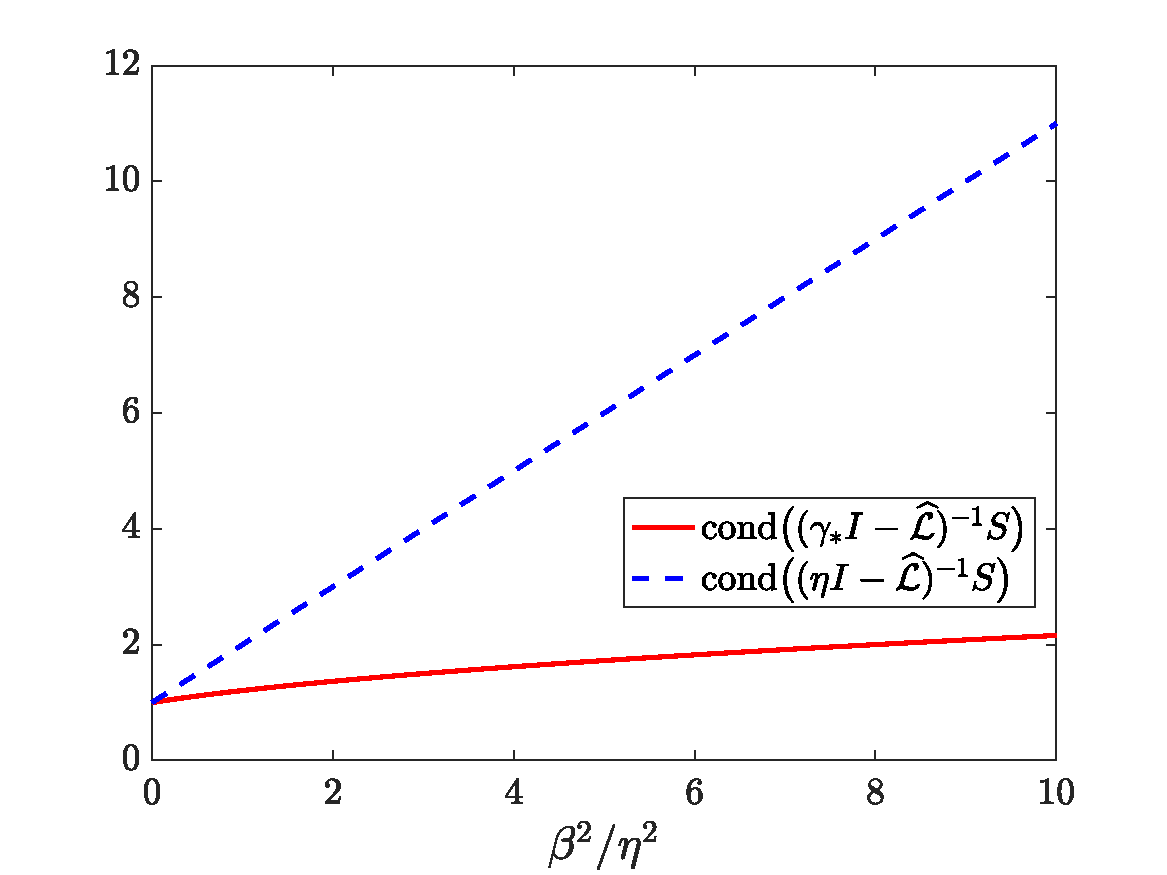
\includegraphics[width = 0.7\textwidth]{conds}
\caption{Optimal ($\gamma = \gamma_*$) and non-optimal ($\gamma = \eta$) condition numbers \eqref{eq:c1_non-opt} and \eqref{eq:cond_min} as a function of $\beta^2/\eta^2$. }
\label{fig:conds}
\end{figure}

\renewcommand{\tabcolsep}{4pt}
\renewcommand{\arraystretch}{1.15}
\begin{table}[!ht]
  \centering
  \begin{tabular}{| c | c | c |}  % chktex 44
  \hline
Method & &  \\ \hline
\multirow{ 3}{*}{Gauss(8)}
&$\beta^2/\eta^2$ & 1.59 / 0.09 \\
&$\gamma = \eta$  -- & 20 / 11\\
&$\gamma = \gamma_*$ & 13 / 11\\ \hline
\multirow{ 3}{*}{Radau IIA(9)}
&$\beta^2/\eta^2$ & 0 / 3.20 / 0.32	\\
&$\gamma = \eta$ &  8 / 24 / 13\\
&$\gamma = \gamma_*$ & 8 / 14/ 11 \\ \hline
\multirow{ 3}{*}{Lobatto IIIC(8)}
&$\beta^2/\eta^2$ & 0 / 4.88 / 0.38 \\
&$\gamma = \eta$ & 8 / 29 / 14\\
&$\gamma = \gamma_*$ & 8 / 15 / 12\\
  \hline
  \end{tabular}
  \caption{
Number of GMRES iterations for each stage when solving $u_t = \Delta u + s$, with a single time step of $\delta t = h = 1/256$. Different values of $\gamma$ are used in the preconditoner, as indicated.
}
\label{tab:cond_iters}
\end{table}

It's interesting to note that $\gamma_*$ does not depend on $\eta$ nor $\beta$. However, note that for $\beta < \eta$, we're unlikely to see any large difference in choosing $\gamma = \eta$ over $\gamma = \gamma_*$:
\begin{align}
\textnormal{cond}\left((\eta I- \widehat{\mathcal{L}})^{-1}S\right)
-
\textnormal{cond}\left((\gamma_* I- \widehat{\mathcal{L}})^{-1}S\right)
=
\frac{3}{4} \left( \frac{\beta}{\eta} \right)^2 + {\cal O}\left( \frac{\beta}{\eta} \right)^4 = {\cal O} \left( \frac{\beta}{\eta} \right)^2.
\end{align}
If using a simplified Newton algorithm, or solving a linear problem using this $2 \times 2$ formulation, one could possibly save some work by setting $\gamma = \eta$ so that the preconditioner for the (1,1) block could also be used on this Schur complement.


% ---------------------------------------------------------------------------------------------- %
% ---------------------------------------------------------------------------------------------- %
\subsection{General conditioning theory}

Consider the more general problem of the \tcb{right} preconditioning 
%
\begin{align}\nonumber
\mathcal{P}_\gamma :&=
S(\gamma I- \widehat{\mathcal{L}}_2)^{-1} \\
& = \left[ (\gamma I - \widehat{\mathcal{L}}_2) + (\eta-\gamma)I +
	\beta^2 (\eta I - \widehat{\mathcal{L}}_1)^{-1}\right]
	(\gamma I - \widehat{\mathcal{L}}_2)^{-1} \\
& = I - (\gamma - \eta)( \gamma I- \widehat{\mathcal{L}}_2)^{-1} + 
	\beta^2( \eta I-\widehat{\mathcal{L}}_1)^{-1}
	( \gamma I- \widehat{\mathcal{L}}_2)^{-1}\nonumber\\
& = I - \frac{\gamma - \eta}{\gamma} ( I- \tfrac{1}{\gamma}\widehat{\mathcal{L}}_2)^{-1} + 
	\frac{\beta^2}{\gamma\eta}( I- \tfrac{1}{\eta}\widehat{\mathcal{L}}_1)^{-1}
	( I- \tfrac{1}{\gamma}\widehat{\mathcal{L}}_2)^{-1},\label{eq:gamma2}
\end{align}




\begin{theorem}[Conditioning of preconditioned operator]\label{th:cond}
Suppose Assumptions \ref{ass:eig} and \ref{ass:fov} hold, that is, $\eta > 0$
and $W(\mathcal{L}) \leq 0$ \eqref{eq:fov}. Additionally, assume that
$\langle\mathcal{L}_1\mathbf{w},\mathcal{L}_2\mathbf{w}\rangle\geq 0$.
Let $\mathcal{P}_\gamma$ denote the right-preconditioned Schur complement,
with preconditioner $(\gamma I - \widehat{\mathcal{L}}_2)^{-1}$, for
$\gamma >\eta$, and define $\gamma_* := \tfrac{\eta^2+\beta^2}{\eta}$.
Then
\begin{align}\label{eq:gammastar}
\textnormal{cond}(\mathcal{P}_{\gamma_*}) \leq 
	2 + \frac{\beta^2}{\eta^2}.
\end{align}
\end{theorem}
\begin{proof}
Recall for matrix $A$, cond$(A) = \|A\|\|A^{-1}\|$.
First, consider bounding $\|(\gamma I- \widehat{\mathcal{L}}_2)^{-1}S\|$ for
$\gamma \geq \eta$:
%
\begin{align}\nonumber
\|\mathcal{P}_\gamma\| & = \left\| I - \frac{\gamma - \eta}{\gamma}
	( I- \tfrac{1}{\gamma}\widehat{\mathcal{L}}_2)^{-1} + 
	\frac{\beta^2}{\gamma\eta}( I- \tfrac{1}{\eta}\widehat{\mathcal{L}}_1)^{-1}
	( I- \tfrac{1}{\gamma}\widehat{\mathcal{L}}_2)^{-1} \right\| \\
% & \leq \left\| I - 2\frac{\gamma-\eta}
% 	{\gamma}\left(I - \tfrac{1}{\gamma}\mathcal{L}\right)^{-1}\right\| +
% 		\frac{\beta^2 + (\gamma-\eta)^2}{\gamma^2}\left\|
% 		\left(I - \tfrac{1}{\gamma}\mathcal{L}\right)^{-2} \right\| \\
& \leq \left\| I - \frac{\gamma-\eta}
	{\gamma}\left(I - \tfrac{1}{\gamma}\mathcal{L}_2\right)^{-1}\right\| +
		\frac{\beta^2}{\gamma\eta}
		\left\|( I- \tfrac{1}{\eta}\widehat{\mathcal{L}}_1)^{-1} \right\|
		\left\|( I- \tfrac{1}{\gamma}\widehat{\mathcal{L}}_2)^{-1}\right\|\nonumber \\
& \leq \left\| I - \frac{\gamma-\eta}
	{\gamma}\left(I - \tfrac{1}{\gamma}\mathcal{L}_2\right)^{-1}\right\| +
		\frac{\beta^2}{\gamma\eta}. \label{eq:Pgn}
\end{align}
%
For the first term, note that maximizing over $\mathbf{v}\in\mathbb{R}^n$ and
letting $\mathbf{v} := (I - \tfrac{1}{\gamma}\mathcal{L}_2)\mathbf{w}$,
%
\begin{align*}
\left\| I - \tfrac{\gamma-\eta}
	{\gamma}(I - \tfrac{1}{\gamma}\mathcal{L}_2)^{-1}\right\|^2
		& = \sup_{\mathbf{v}\neq\mathbf{0}} \frac{\left\| [I - \frac{\gamma-\eta}
	{\gamma}(I - \tfrac{1}{\gamma}\mathcal{L}_2)^{-1}]\mathbf{v}\right\|^2}{\|\mathbf{v}\|^2} 
= \sup_{\mathbf{w}\neq\mathbf{0}} \frac{\left\| (I - \tfrac{1}{\gamma}\mathcal{L}_2 -
		\frac{\gamma-\eta}{\gamma}I )\mathbf{w}\right\|^2}{\|(I - \tfrac{1}{\gamma}\mathcal{L}_2)
		\mathbf{w}\|^2} \\
% & = \sup_{\mathbf{w}\neq\mathbf{0}} \frac{\left\|[(1 - 2\frac{\gamma-\eta}{\gamma})
% 	I - \tfrac{1}{\gamma}\mathcal{L}_2]\mathbf{w}\right\|^2}{\|(I - \tfrac{1}{\gamma}\mathcal{L}_2)
% 		\mathbf{w}\|^2} \\
&\hspace{-5ex} = \sup_{\mathbf{w}\neq\mathbf{0}} \frac{(\tfrac{\eta}{\gamma})^2\|\mathbf{w}\|^2
	- \tfrac{\eta}{\gamma^2}\langle (\mathcal{L}_2 + \mathcal{L}_2^T)
		\mathbf{w},\mathbf{w}\rangle + \tfrac{1}{\gamma}^2\|\mathcal{L}_2\mathbf{w}\|^2}
	{\|\mathbf{w}\|^2 - \tfrac{1}{\gamma}\langle (\mathcal{L}_2 + \mathcal{L}_2^T)
		\mathbf{w},\mathbf{w}\rangle + \tfrac{1}{\gamma}^2\|\mathcal{L}_2\mathbf{w}\|^2}.
\end{align*}
%
Note that by assumption, $\gamma \geq \eta$, which implies
$0< \tfrac{\eta}{\gamma^2} \leq \tfrac{\eta^2}{\gamma^2}  < 1$, and 
$|1 - 2\tfrac{\gamma-\eta}{\gamma}| < 1$. In addition, we assume $W(\mathcal{L}_2)\leq 0$,
which implies $-\langle (\mathcal{L}_2+\mathcal{L}_2^T)\mathbf{w},\mathbf{w}\rangle \geq 0$
(see \Cref{th:fov}). It follows that all terms in the numerator and denominator are
positive, and
%
\begin{align} \label{eq:P1}
\left\| I - \tfrac{\gamma-\eta}
	{\gamma}(I - \tfrac{1}{\gamma}\mathcal{L}_2)^{-1}\right\|^2
& < \sup_{\mathbf{w}\neq\mathbf{0}} \frac{\|\mathbf{w}\|^2
	- \tfrac{1}{\gamma}\langle (\mathcal{L}_2 + \mathcal{L}_2^T)
		\mathbf{w},\mathbf{w}\rangle + \tfrac{1}{\gamma}^2\|\mathcal{L}_2\mathbf{w}\|^2}
	{\|\mathbf{w}\|^2 - \tfrac{1}{\gamma}\langle (\mathcal{L}_2 + \mathcal{L}^T)
		\mathbf{w},\mathbf{w}\rangle + \tfrac{1}{\gamma}^2\|\mathcal{L}\mathbf{w}\|^2} 
= 1.
\end{align}
%
Combining \eqref{eq:P0} and \eqref{eq:P1} yields
%
\begin{align}\label{eq:Pgamma_gen}
\|\mathcal{P}_\gamma\| \leq 1 + \frac{\beta^2}{\gamma\eta}.
\end{align}

Now consider bounding $\|\mathcal{P}_\gamma^{-1}\|$ from above. Let $s_{\max}(A)$
and $s_{\min}(A)$ denote the maximum and minimum singular value of matrix $A$,
respectively, and recall
%
\begin{align*}
\|\mathcal{P}_\gamma^{-1}\| = s_{\max}(\mathcal{P}_\gamma^{-1})
	& = \frac{1}{s_{\min}(\mathcal{P}_\gamma)}, \hspace{5ex}\textnormal{where}\hspace{2ex}
s_{\min}(\mathcal{P}_\gamma) =
	\min_{\mathbf{v}\neq\mathbf{0}} \frac{\|\mathcal{P}_\gamma\mathbf{v}\|}{\|\mathbf{v}\|}.
\end{align*}
%
Thus, consider the minimum singular value of $P_\gamma$. Letting $\mathbf{v} :=
(I - \tfrac{1}{\gamma}\mathcal{L}_2)(I - \tfrac{1}{\eta}\mathcal{L}_1)\mathbf{w}$,
%
\begin{align}\nonumber
s_{\min}(\mathcal{P}_\gamma)^2 & = \min_{\mathbf{v}\neq\mathbf{0}}
	\frac{\left\| \left[I - \frac{\gamma - \eta}{\gamma}
	( I- \tfrac{1}{\gamma}\widehat{\mathcal{L}}_2)^{-1} + 
	\frac{\beta^2}{\gamma\eta}( I- \tfrac{1}{\eta}\widehat{\mathcal{L}}_1)^{-1}
	( I- \tfrac{1}{\gamma}\widehat{\mathcal{L}}_2)^{-1}\right]\mathbf{v} \right\|^2}
	{\|\mathbf{v}\|^2} \\
& = \min_{\mathbf{w}\neq\mathbf{0}}
	\frac{\left\| \left[(I - \tfrac{1}{\gamma}\mathcal{L}_2)(I - \tfrac{1}{\eta}\mathcal{L}_1)
		- \frac{\gamma-\eta}{\gamma}(I - \tfrac{1}{\eta} \mathcal{L}_1) +
		\frac{\beta^2}{\gamma\eta} I\right]\mathbf{w} \right\|^2}
	{\|(I - \tfrac{1}{\gamma}\mathcal{L}_2)(I - \tfrac{1}{\eta}\mathcal{L}_1)\mathbf{w}\|^2} \nonumber\\
& = \min_{\mathbf{w}\neq\mathbf{0}}
	\frac{\left\| \left[(I - \tfrac{1}{\gamma}\mathcal{L}_2)(I - \tfrac{1}{\eta}\mathcal{L}_1)
		+ \frac{\gamma-\eta}{\gamma\eta}\mathcal{L}_1 +
		\frac{\beta^2+\eta^2 - \gamma\eta}{\gamma\eta} I\right]\mathbf{w} \right\|^2}
	{\|(I - \tfrac{1}{\gamma}\mathcal{L}_2)(I - \tfrac{1}{\eta}\mathcal{L}_1)\mathbf{w}\|^2} \nonumber
\end{align}
%
Let us make the strategic choice of picking $\gamma$ such that the identity perturbation
$\tfrac{\beta^2+\eta^2 - \gamma\eta}{\gamma\eta} I = \mathbf{0}$, given by $\gamma_*
:= \tfrac{\eta^2+\beta^2}{\eta}$. Note, this is exactly the optimal $\gamma$ in the case
of SPD operators $\mathcal{L}$. Expanding, we have
%
\begin{align}
s_{\min}(\mathcal{P}_\gamma)^2 & = 
	\min_{\mathbf{w}\neq\mathbf{0}}
	\frac{\left\| \left[(I - \tfrac{1}{\gamma}\mathcal{L}_2)(I - \tfrac{1}{\eta}\mathcal{L}_1)
		+ \frac{\beta^2}{\eta(\eta^2+\beta^2)}\mathcal{L}_1\right]\mathbf{w} \right\|^2}
	{\|(I - \tfrac{1}{\gamma}\mathcal{L}_2)(I - \tfrac{1}{\eta}\mathcal{L}_1)\mathbf{w}\|^2} \nonumber\\
& = \min_{\mathbf{w}\neq\mathbf{0}} 1 +
	\frac{\beta^2}{\eta(\eta^2+\beta^2)}\cdot 
	\frac{\frac{\beta^2}{\eta(\eta^2+\beta^2)}\left\|\mathcal{L}_1\mathbf{w} \right\|^2
		+ 2\left\langle(I - \tfrac{1}{\gamma}\mathcal{L}_2)(I - \tfrac{1}{\eta}\mathcal{L}_1)\mathbf{w},
		\mathcal{L}_1\mathbf{w} \right\rangle}
	{\|(I - \tfrac{1}{\gamma}\mathcal{L}_2)(I - \tfrac{1}{\eta}\mathcal{L}_1)\mathbf{w}\|^2} \nonumber\\
& = 1 - \frac{\beta^2}{\eta^2+\beta^2} \cdot\max_{\mathbf{w}\neq\mathbf{0}}
	\frac{(-\tfrac{2}{\eta})\left\langle(I - \tfrac{1}{\gamma}\mathcal{L}_2)(I -
		\tfrac{1}{\eta}\mathcal{L}_1)\mathbf{w},
		\mathcal{L}_1\mathbf{w} \right\rangle- 
		\frac{\beta^2}{\eta^2(\eta^2+\beta^2)}\left\|\mathcal{L}_1\mathbf{w} \right\|^2}
	{\|(I - \tfrac{1}{\gamma}\mathcal{L}_2)(I - \tfrac{1}{\eta}\mathcal{L}_1)\mathbf{w}\|^2}.
	\label{eq:gen_smin}
\end{align}
%
Expanding the numerator term, we have
\begin{align}\nonumber
& (-\tfrac{2}{\eta})\left\langle(I - \tfrac{1}{\gamma}\mathcal{L}_2)(I - \tfrac{1}{\eta}\mathcal{L}_1)\mathbf{w},
		\mathcal{L}_1\mathbf{w} \right\rangle- 
		\frac{\beta^2}{\eta^2(\eta^2+\beta^2)}\left\|\mathcal{L}_1\mathbf{w} \right\|^2 \\
& = \left(\frac{2}{\eta^2} - \frac{\beta^2}{\eta^2(\eta^2+\beta^2)}\right)
			\left\|\mathcal{L}_1\mathbf{w} \right\|^2
		- \frac{2}{\eta}\langle\mathbf{w},\mathcal{L}_1\mathbf{w}\rangle
		- \frac{2}{\gamma\eta^2}\langle\mathcal{L}_2(\mathcal{L}_1\mathbf{w}),\mathcal{L}_1\mathbf{w}\rangle
		+ \frac{2}{\gamma\eta}\langle\mathcal{L}_1\mathbf{w},\mathcal{L}_2\mathbf{w}\rangle \nonumber\\
& = \left(\frac{1}{\eta^2} + \frac{1}{\eta^2+\beta^2}\right)
			\left\|\mathcal{L}_1\mathbf{w} \right\|^2
		- \frac{2}{\eta}\langle\mathbf{w},\mathcal{L}_1\mathbf{w}\rangle
		- \frac{2}{\gamma\eta^2}\langle\mathcal{L}_2(\mathcal{L}_1\mathbf{w}),\mathcal{L}_1\mathbf{w}\rangle
		+ \frac{2}{\gamma\eta}\langle\mathcal{L}_1\mathbf{w},\mathcal{L}_2\mathbf{w}\rangle.
		\label{eq:num_gen}
\end{align}
%
Now consider the denominator:
%
\begin{align}
\left\|(I - \tfrac{1}{\gamma}\mathcal{L}_2)(I - \tfrac{1}{\eta}\mathcal{L}_1)\mathbf{w}\right\|^2
& = \left\|\left(I + \tfrac{1}{\gamma\eta}\mathcal{L}_2\mathcal{L}_1\right)\mathbf{w} - 
	\left(\tfrac{1}{\gamma}\mathcal{L}_2 + \tfrac{1}{\eta}\mathcal{L}_1\right)\mathbf{w}\right\|^2 \nonumber\\
& = \left\|\left(I + \tfrac{1}{\gamma\eta}\mathcal{L}_2\mathcal{L}_1\right)\mathbf{w}\right\|^2
	+ \frac{1}{\gamma^2}\|\mathcal{L}_2\mathbf{w}\|^2
	+ \frac{1}{\eta^2}\|\mathcal{L}_1\mathbf{w}\|^2
	+ \frac{2}{\gamma\eta}\langle\mathcal{L}_1\mathbf{w},\mathcal{L}_2\mathbf{w}\rangle
	\nonumber\\ & \hspace{5ex}
	- \frac{2}{\gamma}\Big\langle \left(I + \tfrac{1}{\gamma\eta}\mathcal{L}_2\mathcal{L}_1\right)\mathbf{w},
		\mathcal{L}_2\mathbf{w}\Big\rangle
	- \frac{2}{\eta}\Big\langle \left(I + \tfrac{1}{\gamma\eta}\mathcal{L}_2\mathcal{L}_1\right)\mathbf{w},
		\mathcal{L}_1\mathbf{w}\Big\rangle \nonumber\\
& \geq \left\|\left(I + \tfrac{1}{\gamma\eta}\mathcal{L}_2\mathcal{L}_1\right)\mathbf{w}\right\|^2
	+ \frac{1}{\gamma^2}\|\mathcal{L}_2\mathbf{w}\|^2
	+ \frac{1}{\eta^2}\|\mathcal{L}_1\mathbf{w}\|^2
	+ \frac{2}{\gamma\eta}\langle\mathcal{L}_1\mathbf{w},\mathcal{L}_2\mathbf{w}\rangle
	\nonumber\\ & \hspace{5ex}
	- \frac{2}{\gamma}\left\| \left(I + \tfrac{1}{\gamma\eta}\mathcal{L}_2\mathcal{L}_1\right)\mathbf{w}\right\|
		\left\|\mathcal{L}_2\mathbf{w}\right\|
	- \frac{2}{\eta}\Big\langle \left(I + \tfrac{1}{\gamma\eta}\mathcal{L}_2\mathcal{L}_1\right)\mathbf{w},
		\mathcal{L}_1\mathbf{w}\Big\rangle \nonumber\\
& = \left( \left\|\left(I + \tfrac{1}{\gamma\eta}\mathcal{L}_2\mathcal{L}_1\right)\mathbf{w}\right\|
		- \frac{1}{\gamma}\|\mathcal{L}_2\mathbf{w}\|\right)^2
	+ \frac{1}{\eta^2}\|\mathcal{L}_1\mathbf{w}\|^2
	\nonumber\\ & \hspace{5ex}
	- \frac{2}{\eta}\Big\langle \left(I + \tfrac{1}{\gamma\eta}\mathcal{L}_2\mathcal{L}_1\right)\mathbf{w},
		\mathcal{L}_1\mathbf{w}\Big\rangle
	+ \frac{2}{\gamma\eta}\langle\mathcal{L}_1\mathbf{w},\mathcal{L}_2\mathbf{w}\rangle \nonumber\\
& \geq \frac{1}{\eta^2}\|\mathcal{L}_1\mathbf{w}\|^2
	- \frac{2}{\eta}\langle \mathbf{w}, \mathcal{L}_1\mathbf{w}\Big\rangle 
	- \frac{2}{\gamma\eta^2}\langle \mathcal{L}_2(\mathcal{L}_1\mathbf{w}),
		\mathcal{L}_1\mathbf{w}\Big\rangle
	+ \frac{2}{\gamma\eta}\langle\mathcal{L}_1\mathbf{w},\mathcal{L}_2\mathbf{w}\rangle.
		\label{eq:den_gen}
\end{align}
%

By assumption $\langle\mathcal{L}_1\mathbf{w},\mathcal{L}_2\mathbf{w}\rangle\geq 0$,
and thus all terms in \eqref{eq:num_gen} and \eqref{eq:den_gen} are non-negative.
Returning to the minimum singular value defined in \eqref{eq:gen_smin} and plugging in
the numerator \eqref{eq:num_gen} and denominator bounds \eqref{eq:den_gen} yields
an upper bound on the maximum over $\mathbf{w}$,
%
\begin{align*}
&\hspace{-5ex} \max_{\mathbf{w}\neq\mathbf{0}}
	\frac{(-\tfrac{2}{\eta})\left\langle(I - \tfrac{1}{\gamma}\mathcal{L}_2)(I -
		\tfrac{1}{\eta}\mathcal{L}_1)\mathbf{w},
		\mathcal{L}_1\mathbf{w} \right\rangle- 
		\frac{\beta^2}{\eta^2(\eta^2+\beta^2)}\left\|\mathcal{L}_1\mathbf{w} \right\|^2}
	{\|(I - \tfrac{1}{\gamma}\mathcal{L}_2)(I - \tfrac{1}{\eta}\mathcal{L}_1)\mathbf{w}\|^2} \\
& \leq \max_{\mathbf{w}\neq\mathbf{0}}\frac{\left(\frac{1}{\eta^2} + \frac{1}{\eta^2+\beta^2)}\right)
			\left\|\mathcal{L}_1\mathbf{w} \right\|^2
		- \frac{2}{\eta}\langle\mathbf{w},\mathcal{L}_1\mathbf{w}\rangle
		- \frac{2}{\gamma\eta^2}\langle\mathcal{L}_2(\mathcal{L}_1\mathbf{w}),\mathcal{L}_1\mathbf{w}\rangle
		+ \frac{2}{\gamma\eta}\langle\mathcal{L}_1\mathbf{w},\mathcal{L}_2\mathbf{w}\rangle}
	{\frac{1}{\eta^2}\|\mathcal{L}_1\mathbf{w}\|^2
	- \frac{2}{\eta}\langle \mathbf{w}, \mathcal{L}_1\mathbf{w}\Big\rangle 
	- \frac{2}{\gamma\eta^2}\langle \mathcal{L}_2(\mathcal{L}_1\mathbf{w}),
		\mathcal{L}_1\mathbf{w}\Big\rangle
	+ \frac{2}{\gamma\eta}\langle\mathcal{L}_1\mathbf{w},\mathcal{L}_2\mathbf{w}\rangle} \nonumber\\
& \leq \frac{\frac{1}{\eta^2} + \frac{1}{\eta^2+\beta^2)}}{\frac{1}{\eta^2}} \\
& = \frac{2\eta^2 + \beta^2}{\eta^2+\beta^2}.
\end{align*}
%
Plugging in to \eqref{eq:gen_smin} yields
%
\begin{align}
s_{\min}(\mathcal{P}_{\gamma_*})^2 &\geq 1 - \frac{\beta^2}{\eta^2+\beta^2}
	\frac{2\eta^2 + \beta^2}{\eta^2+\beta^2}
= \frac{\eta^4}{(\eta^2+\beta^2)^2}.
\end{align}
%
Combing with \eqref{eq:Pgamma_gen} yields
%
\begin{align}
\textnormal{cond}(\mathcal{P}_{\gamma_*}) = \|\mathcal{P}_{\gamma_*}\|\|\mathcal{P}_{\gamma_*}^{-1}\|
	\leq \left(1+\frac{\eta^2}{\eta^2+\beta^2}\right)\frac{\eta^2+\beta^2}{\eta^2}
	= 2+\frac{\beta^2}{\eta^2},
\end{align}
%
which completes the proof.
\end{proof}
%




\end{document}


 
% % ---------------------------------------------------------------------------------------------- %
% % ---------------------------------------------------------------------------------------------- %
% % ---------------------------------------------------------------------------------------------- %
% \section{A better constant}

% {\color{blue}
% \textbf{This section is outdated and did not yield anything useful.}
% }


% Note that for real $k>0$, $W\left[\left(I - \tfrac{1}{k}\mathcal{L}\right)^{-1}\right]$ and
% $W\left[\left(I - \tfrac{1}{k}\mathcal{L}\right)^{-2}\right]$ are contained in
% the positive half unit circle. Now consider the more general preconditioning
% %
% \begin{align}\nonumber
% (kI - \mathcal{L})^{-2}\Big[(nI - \mathcal{L})^2 + \beta^2 I\Big] 
% 	& = (kI - \mathcal{L})^{-2}\Big[(\eta-k)I + (kI - \mathcal{L}))^2 + \beta^2 I\Big] \\
% & = (kI - \mathcal{L})^{-2}\Big[(k-\eta)^2I - 2(k-\eta)(kI - \mathcal{L}) + (kI - \mathcal{L})^2 + \beta^2 I\Big] \nonumber\\
% & = I - 2(k-\eta)(kI - \mathcal{L})^{-1} + (\beta^2 + (k-\eta)^2)(kI - \mathcal{L})^{-2} \nonumber\\
% & = I - 2\frac{k-\eta}{k}\left(I - \tfrac{1}{k}\mathcal{L}\right)^{-1} + \frac{\beta^2 + (k-\eta)^2}{k^2}
% 	\left(I - \tfrac{1}{k}\mathcal{L}\right)^{-2}.\label{eq:gen1}
% \end{align}
% %
% Note that we have a quadratic polynomial in $\left(I - \tfrac{1}{k}\mathcal{L}\right)^{-1}$.
% Working out the roots of the corresponding polynomial, one can see they come in
% conjugate pairs,
% %
% \begin{align*}
% \frac{ 2\frac{k-\eta}{k} \pm \sqrt{4\frac{(k-\eta)^2}{k^2} - 4\frac{\beta^2}{k^2} -
% 	4\frac{(k-\eta)^2}{k^2}}}{ 2\frac{\beta^2 + (k-\eta)^2}{k^2}} 
% = \frac{k(k-\eta) \pm \mathrm{i} k\beta}{\beta^2 + (k-\eta)^2}.
% \end{align*}
% %
% Let $\alpha$ denote the inverse of thees roots. Then \eqref{eq:gen1} can
% be expressed in factored form as
% %
% \begin{align*}
% (kI - \mathcal{L})^{-2}\Big[(nI - \mathcal{L})^2 + \beta^2 I\Big] 
% 	& = \Big[I - \overline{\alpha}\left(I - \tfrac{1}{k}\mathcal{L}\right)^{-1}\Big]
% 	\Big[I - \alpha\left(I - \tfrac{1}{k}\mathcal{L}\right)^{-1}\Big],
% \end{align*}
% %
% where $\alpha + \overline{\alpha} = 2\tfrac{k-\eta}{k}$ and $\alpha\overline{\alpha}
% = \tfrac{\beta^2 + (k-\eta)^2}{k^2}$. For ease of notation, let us denote
% $\mathcal{P} := \left(I - \tfrac{1}{k}\mathcal{L}\right)^{-1}$,
% and consider the field of values of 
% %
% \begin{align*}
% \mathcal{Z} := (I - \overline{\alpha}\mathcal{P})(I - {\alpha}\mathcal{P}).
% \end{align*}
% %

% We start by considering the real part of $\mathcal{Z}$ to bound the FOV along the real axis,
% %
% \begin{align*}
% \frac{1}{2}(\mathcal{Z} + \mathcal{Z}^*)
% 	& = \frac{1}{2}\Big[ 2I - (\alpha + \overline{\alpha})(\mathcal{P}+\mathcal{P}^T) +
% 		\alpha\overline{\alpha}(\mathcal{P}^2 + (\mathcal{P}^T)^2)\Big] \\
% & = \frac{1}{2}\Big[ \Big(I - (\alpha + \overline{\alpha})(\mathcal{P}+\mathcal{P}^T) +
% 		\alpha\overline{\alpha}(\mathcal{P} + \mathcal{P}^T)^2\Big) +
% 		\Big(I - \alpha\overline{\alpha}(\mathcal{P}\mathcal{P}^T + \mathcal{P}^T\mathcal{P})\Big) \Big].
% \end{align*}
% %
% Note that $(\mathcal{P}+\mathcal{P}^T)$, $\mathcal{P}\mathcal{P}^T$, and
% $\mathcal{P}^T\mathcal{P}$ are all SPD with eigenvalues $\lambda\in(0,2)$
% for $(\mathcal{P}+\mathcal{P}^T)$ and $\lambda\in(0,1)$ for the others.
% If $\mathcal{P}=\mathcal{P}^T$ is symmetric, the two operators above would
% share eigenvectors as well, and we could get tighter bounds. As is, we have
% to assume worst case that the eigenvectors of
% $\mathcal{P}^T\mathcal{P} + \mathcal{P}\mathcal{P}^T$ corresponding to the
% largest eigenvalues correspond to the smallest of $(\mathcal{P}+\mathcal{P}^T$,
% and vice versa. In this case, we have bounds 
% %
% \begin{align}
% \lambda_{\max}\left(\frac{1}{2}(\mathcal{Z} + \mathcal{Z}^*)\right) & \leq 
% 	\frac{1}{2}\Big(2 - (\alpha + \overline{\alpha})\lambda +
% 		\alpha\overline{\alpha}\lambda^2\Big) \label{eq:lam_max}.
% % & = \frac{1}{2}\Big(1 + (1 -\alpha\lambda)(1 -\overline{\alpha}\lambda)\Big).
% \end{align}
% %
% for $\lambda\in(0,2)$. Finding the critical point $\lambda_* =
% \tfrac{\alpha+\overline{\alpha}}{2\alpha\overline{\alpha}}$, the maximum will
% be obtained at be evaluating \eqref{eq:lam_max} for $\lambda\in\{0,2,\lambda_*\}$.
% Note, the difference between here and the symmetric case is for symmetric we only
% evaluate to $\lambda = 1$ I think.

% Letting $k := \sqrt{\eta^2+\beta^2}$, we have
% %
% \begin{align*}
% \alpha + \overline{\alpha} & = 2\frac{\sqrt{\eta^2+\beta^2} - \eta}{\sqrt{\eta^2+\beta^2}}
% 	= 2 - 2\frac{\eta}{\sqrt{\eta^2+\beta^2}}, \\
% |\alpha|^2 & = \alpha\overline{\alpha} = \frac{\beta^2 + \left(\sqrt{\eta^2+\beta^2} - \eta\right)^2}{\eta^2+\beta^2} \\
% & = 2 - 2\frac{\eta}{\sqrt{\eta^2+\beta^2}}.
% \end{align*}
% %
% Noting that here we have $\alpha + \overline{\alpha} = \alpha\overline{\alpha}$, 
% \eqref{eq:lam_max} simplifies to
% %
% \begin{align*}
% \lambda_{\max}\left(\frac{1}{2}(\mathcal{Z} + \mathcal{Z}^*)\right) & \leq 
% 	\frac{1}{2}\Big(2 + \alpha \overline{\alpha}(\lambda^2 - \lambda)\Big),
% \end{align*}
% %
% and $\lambda_* = \frac{\alpha + \overline{\alpha}}{2\alpha\overline{\alpha}} = \frac{1}{2}$.
% Evaluating \eqref{eq:lam_max} at $\lambda\in\{0,2,\lambda_*\}$, where now
% $\lambda_* = \tfrac{1}{2}$, yields
% %
% \begin{align*}
% \lambda & = 0 \mapsto \frac{1}{2}(2), \\
% \lambda & = 1 \mapsto \frac{1}{2}(2), \\
% \lambda & = 2 \mapsto 3 - \frac{\eta}{\sqrt{\eta^2+\beta^2}}, \\
% \lambda_* & = \frac{1}{2} \mapsto \frac{1}{2}\Big(\frac{3}{2} + \frac{\eta}{2\sqrt{\eta^2+\beta^2}} \Big)
% \end{align*}
% %

% For the minimum eigenvalue, the best we can do is
% %
% \begin{align}
% \lambda_{\min}\left(\frac{1}{2}(\mathcal{Z} + \mathcal{Z}^*)\right) & \geq 
% 	\frac{1}{2}\Big(2 - (\alpha + \overline{\alpha})\lambda +
% 		\alpha\overline{\alpha}\lambda^2 - 2\alpha\overline{\alpha}\Big) \nonumber\\
% & = \frac{1}{2}\Big(2 + \alpha\overline{\alpha}(\lambda^2 - \lambda - 2)\Big).\label{eq:lam_min}
% \end{align}
% %
% Here we again have a critical point at $\lambda_* = \tfrac{1}{2}$. Evaluating
% \eqref{eq:lam_min} yields
% %
% \begin{align*}
% \lambda & = 0 \mapsto -1 + 2\frac{\eta}{\sqrt{\eta^2+\beta^2}}, \\
% \lambda & = 1 \mapsto -1 + 2\frac{\eta}{\sqrt{\eta^2+\beta^2}}, \\
% \lambda & = 2 \mapsto \frac{1}{2}(2), \\
% \lambda_* & = \frac{1}{2} \mapsto 
% \end{align*}
% %

% {\color{blue}0 and 1 only positive for $\beta < \sqrt{3}\eta$ =(.

% Current approach can be seen as using spectral equivalence
% %
% \begin{align*}
% P^2 + (P^T)^2 & = (P+P^T)^2 - (PP^T + P^TP) \geq (P+P^T)^2.
% \end{align*}
% %
% This is too rough of an estimate. Need better spectral equivalence
% to replace 

% }

% % ---------------------------------------------------------------------------------------------- %
% % ---------------------------------------------------------------------------------------------- %
% % ---------------------------------------------------------------------------------------------- %
% \section{Tom}

% Let $\eta,\beta > 0$ be real constants and $\mathcal{L}$ a spatial operator with
% negative field of values, $W(\mathcal{L} \leq 0$. Now suppose we want to precondition
% the quadratic polynomial in $\mathcal{L}$,
% %
% \begin{align*}
% Q := (\eta I - \mathcal{L})^2 + \beta^2 I.
% \end{align*}
% %
% I derived some nice field of values analysis that shows using
% %
% \begin{align*}
% P_\eta := (\eta I - \mathcal{L})^{-2}
% \end{align*}
% %
% results in a nicely bounded field of values show below:
% %
% \begin{figure}[h!]
% \centering
% 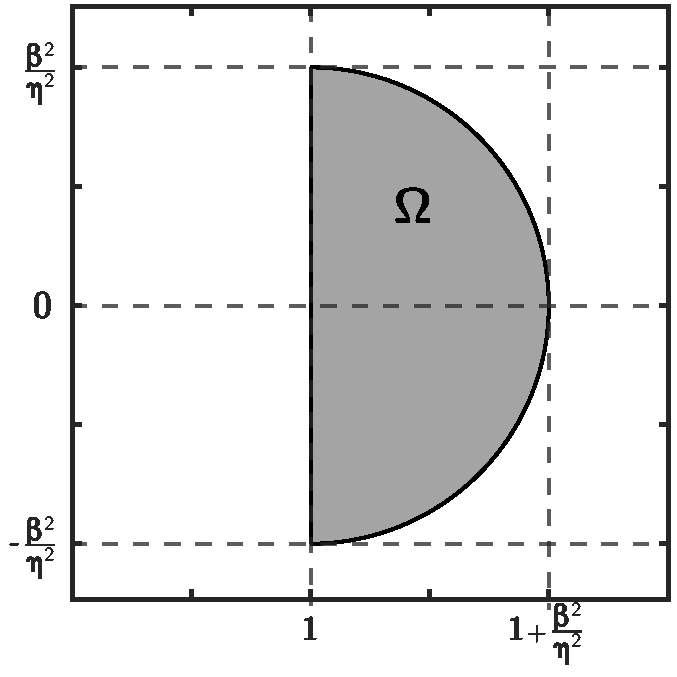
\includegraphics[width = 0.3\textwidth]{./fov_fig.pdf}
% \caption{}
% \label{fig:bound}
% \end{figure}
% %

% However, $\eta$ is probably not the best constant to use. For SPD matrices, 
% somebody proved that using a constant $k := \sqrt{\eta^2+\beta^2}$ and
% preconditioner
% %
% \begin{align*}
% P_k := (k I - \mathcal{L})^{-2}
% \end{align*}
% %
% is a much better choice for $\beta \gg \eta$. I am trying to figure out if
% anything similar can be said for the FOV (or other more general types of
% analysis/operator).

% Note that for real $k>0$, $W\left[\left(I - \tfrac{1}{k}\mathcal{L}\right)^{-1}\right]$ and
% $W\left[\left(I - \tfrac{1}{k}\mathcal{L}\right)^{-2}\right]$ are contained in
% the positive half unit circle. Now consider the more general preconditioning
% %
% \begin{align}\nonumber
% (kI - \mathcal{L})^{-2}\Big[(nI - \mathcal{L})^2 + \beta^2 I\Big] 
% 	& = (kI - \mathcal{L})^{-2}\Big[(\eta-k)I + (kI - \mathcal{L}))^2 + \beta^2 I\Big] \\
% & = (kI - \mathcal{L})^{-2}\Big[(k-\eta)^2I - 2(k-\eta)(kI - \mathcal{L}) + (kI - \mathcal{L})^2 + \beta^2 I\Big] \nonumber\\
% & = I - 2(k-\eta)(kI - \mathcal{L})^{-1} + (\beta^2 + (k-\eta)^2)(kI - \mathcal{L})^{-2} \nonumber\\
% & = I - 2\frac{k-\eta}{k}\left(I - \tfrac{1}{k}\mathcal{L}\right)^{-1} + \frac{\beta^2 + (k-\eta)^2}{k^2}
% 	\left(I - \tfrac{1}{k}\mathcal{L}\right)^{-2}.\label{eq:gen0}
% \end{align}
% %
% Note that we have a quadratic polynomial in $\left(I - \tfrac{1}{k}\mathcal{L}\right)^{-1}$.
% Let $\alpha$ denote the inverse of the roots of the corresponding polynomial.
% Then \eqref{eq:gen1} can be expressed in factored form as
% %
% \begin{align*}
% (kI - \mathcal{L})^{-2}\Big[(nI - \mathcal{L})^2 + \beta^2 I\Big] 
% 	& = \Big[I - \overline{\alpha}\left(I - \tfrac{1}{k}\mathcal{L}\right)^{-1}\Big]
% 	\Big[I - \alpha\left(I - \tfrac{1}{k}\mathcal{L}\right)^{-1}\Big],
% \end{align*}
% %
% where $\alpha + \overline{\alpha} = 2\tfrac{k-\eta}{k}$ and $\alpha\overline{\alpha}
% = \tfrac{\beta^2 + (k-\eta)^2}{k^2}$. For ease of notation, let us denote
% $\mathcal{P} := \left(I - \tfrac{1}{k}\mathcal{L}\right)^{-1}$.
% {\color{blue}
% We are now interested in the field of values of 
% %
% \begin{align*}
% \mathcal{Z} := (I - \overline{\alpha}\mathcal{P})(I - {\alpha}\mathcal{P}).
% \end{align*}
% %
% where $W(\mathcal{P})$ is contained in the positive half of the unit circle.
% This seems like a nice structure and operator, but I'm stuck. I've tried the
% standard symmetric and skew symmetric splittings. The symmetric works okay for
% an opper bound, but I cannot get a lower bound $> 0$. This is all related to
% \eqref{eq:gen0}, in particular how $\langle \mathcal{P}\mathbf{x},\mathbf{x}\rangle$
% and $\langle \mathcal{P}^2\mathbf{x},\mathbf{x}\rangle$ relate? In general I know
% the FOV of $A$ and $A^2$ don't necessarily relate, but there's a lot of nice
% structure here, and numerical results make $k = \sqrt{\eta^2+\beta^2}$ seem
% optimal for very nonsymmetric advective matrices as well.
% }


% % ------------------------------------------------------------------- %
% % ------------------------------ WRONG ------------------------------
% % ------------------------------------------------------------------- %
% \section{Old analysis different consatnts, SPD operators}

% \tcr{THIS IS WRONG BECAUSE CANNOT POSE AS QUADRATIC POLYNOMIAL WITH DIFFERENT CONSTANTS}

% Suppose $\widehat{\mathcal{L}}$ is symmetric negative definite and, thus, has an orthogonal
% basis of eigenvectors, and consider the conditioning of \eqref{eq:gamma0}. Assume that the
% eigenvalues of $( I- \tfrac{1}{\eta}\widehat{\mathcal{L}})^{-1} \subset (0,1)$, and are
% somewhat dense in this interval. This is to be expected for parabolic problems, where the
% eigenvalues of $-\widehat{\mathcal{L}}$ range from $\sim \delta t$ to $\sim \delta t/h^2$,
% which typically corresponds to $\sim(0,\infty)$ as $h,\delta t\to 0$.

% Note that \eqref{eq:gamma0} is a quadratic polynomial in an SPD operator, and the
% eigenvalues of \eqref{eq:gamma0} are then a quadratic function $P(\lambda)$ of the
% eigenvalues $\{\lambda\}$ of $\widehat{\mathcal{L}}$, where
% %
% \begin{align}\label{eq:quadratic}
% P(\lambda,\gamma) &:= \frac{\beta^2}{\gamma\eta}\lambda^2 - \frac{\gamma - \eta}{\gamma}\lambda + 1.
% \end{align}
% %
% Assume that we choose $\gamma$ such that \eqref{eq:gamma0} is also SPD (choosing otherwise
% would be a poor choice in terms of conditioning). Then the condition number of
% \eqref{eq:gamma0} is given by
% %
% \begin{align}\label{eq:cond0}
% \textnormal{cond}\left((\gamma I- \widehat{\mathcal{L}})^{-1}S\right) & =
% 	\frac{\lambda_{\max}\left((\gamma I- \widehat{\mathcal{L}})^{-1}S\right)}
% 		{\lambda_{\min}\left((\gamma I- \widehat{\mathcal{L}})^{-1}S\right)}.
% \end{align}
% %
% Again assuming that eigenvalues $\lambda\in\sigma\left(\widehat{\mathcal{L}}\right)$ take
% on values $\lambda\in(0,1)$, the condition number \eqref{eq:cond0} can be expressed
% precisely as $h,\delta t\to 0$ via
% %
% \begin{align}\label{eq:cond1}
% \textnormal{cond}\left((\gamma I- \widehat{\mathcal{L}})^{-1}S\right) & =
% 	\frac{\max_{x\in(0,1)} P(x,\gamma)}{\min_{y\in(0,1)} P(y,\gamma)}.
% \end{align}
% %
% With this closed form, it is natural to pose a minimization problem to find the
% optimal $\gamma$ in terms of minimizing the condition number \eqref{eq:cond0}.
% We make the assumption that $\eta \leq \gamma \leq \eta^2+\beta^2$, and consider
% the problem
% %
% \begin{align*}
% \gamma_* & = \textnormal{argmin}_{\gamma \geq \eta}
% 	\frac{\max_{x\in(0,1)} P(x,\gamma)}{\min_{y\in(0,1)} P(y,\gamma)}.
% \end{align*}
% %

% For $\gamma > 0$, $P(\lambda,\gamma)$ is concave up in $\lambda$, and thus
% the maximum over a closed interval $[0,1]$ will be obtained at one of the
% end points,
% %
% \begin{align*}
% P(0) = 1, \hspace{5ex} P(1) = \frac{\eta^2+\beta^2}{\eta\gamma}.
% \end{align*}
% %
% For the maximum eigenvalue, this yields
% %
% \begin{align}\label{eq:max0}
% \lambda_{\max} & = \begin{cases} 
% 	\frac{\eta^2+\beta^2}{\gamma\eta} & \gamma\leq \frac{\eta^2+\beta^2}{\eta}, \\
% 	1 & \gamma > \frac{\eta^2+\beta^2}{\eta}.
% 	\end{cases}
% \end{align}
% %
% If there is a critical point within the interval $(0,1)$, the minimum
% will be obtained at this critical point, otherwise it will be obtained
% at the other endpoint (i.e., not where the maximum is obtained). Solving
% for $\tfrac{\partial P(\lambda,\gamma)}{\lambda}$ and setting equal to
% zero, we have a root
% %
% \begin{align*}
% \lambda_0 := \frac{\eta(\gamma-\eta)}{ 2\beta^2} \geq 0, \hspace{5ex}
% P(\lambda_0,\gamma) & = 1 - \frac{\eta(\gamma-\eta)^2}{4\beta^2\gamma},
% \end{align*}
% %
% which satisfies $\lambda_0<1$ when $\gamma < \tfrac{2\beta^2+\eta^2}{\eta}$.
% If we suppose $\lambda_0<1$, we have 
% %
% \begin{align}\label{eq:min0}
% \lambda_{\min} & = P(\lambda_0,\gamma) = 1 - \frac{\eta(\gamma-\eta)^2}{4\beta^2\gamma}.
% \end{align}
% %
% For $\gamma \geq \tfrac{\eta^2+2\beta^2}{\eta} > \tfrac{\eta^2+\beta^2}{\eta}$,
% from \eqref{eq:max0}, we have $\lambda_{\min} = \frac{\eta^2+\beta^2}{\gamma\eta}$.
% Altogether, we have the condition number as a continuous function of $\gamma$,
% %
% \begin{align}\label{eq:cases}
% \textnormal{cond}\left((\gamma I- \widehat{\mathcal{L}})^{-1}S\right) & =
% % 	\begin{cases}
% % 		\frac{\frac{\eta^2+\beta^2}{\gamma\eta}}{1 - \frac{\eta(\gamma-\eta)^2}{4\beta^2\gamma}}
% % 			& \gamma\leq \frac{\eta^2+\beta^2}{\eta}, \\
% % 		\frac{1}{1 - \frac{\eta(\gamma-\eta)^2}{4\beta^2\gamma}}
% % 			& \frac{\eta^2+\beta^2}{\eta} \leq \gamma\leq \frac{\eta^2+2\beta^2}{\eta}, \\
% % 		\frac{1}{\frac{\eta^2+\beta^2}{\gamma\eta}}
% % 			& \frac{\eta^2+2\beta^2}{\eta} \leq \gamma.
% % 	\end{cases}
% % \\ & = \textnormal{argmin}_{\gamma \in[\eta,\eta^2+\beta^2]} 
% 	\begin{cases}
% 		\frac{4\beta^2(\eta^2+\beta^2)}{4\beta^2\gamma\eta - \eta^2(\gamma-\eta)^2}
% 			& \eta \leq \gamma< \frac{\eta^2+\beta^2}{\eta}, \\
% 		\frac{4\beta^2\gamma}{4\beta^2\gamma - \eta(\gamma-\eta)^2}
% 			& \frac{\eta^2+\beta^2}{\eta} \leq \gamma < \frac{\eta^2+2\beta^2}{\eta}, \\
% 		\frac{\gamma\eta}{\eta^2+\beta^2}
% 			& \frac{\eta^2+2\beta^2}{\eta} \leq \gamma.
% 	\end{cases}
% \end{align}
% %
% To proceed with the proof, we consider each of these cases individually.\\
% \\
% \underline{$\mathbf{\frac{\boldsymbol{\eta}^2+2\boldsymbol{\beta}^2}{\boldsymbol{\eta}}
% 	\leq \boldsymbol{\gamma}:}$}
% This is the simplest case. Simply note that for $0<\eta\leq \gamma$,
% %
% \begin{align*}
% \frac{\partial}{\partial\gamma} \left[\frac{\gamma\eta}{\eta^2+\beta^2}\right] = 
% 	\frac{\eta}{\eta^2+\beta^2} > 0,
% \end{align*}
% %
% and thus the minimum value for $\gamma \geq \frac{\eta^2+2\beta^2}{\eta}$ is
% obtained at the lower point of the interval, $\gamma = \frac{\eta^2+2\beta^2}{\eta}$.\\
% \\
% \underline{$\mathbf{\frac{\boldsymbol{\eta}^2+\boldsymbol{\beta}^2}{\boldsymbol{\eta}} \leq
% 	\boldsymbol{\gamma} < \frac{\boldsymbol{\eta}^2+2\boldsymbol{\beta}^2}{\boldsymbol{\eta}}}$:}
% Taking the derivative with respect to $\gamma$ from the appropriate equation in
% \eqref{eq:cases}, we get nice cancellation to arrive at
% %
% \begin{align*}
% \frac{\partial}{\partial\gamma} \left[\frac{4\beta^2\gamma}{4\beta^2\gamma - \eta(\gamma-\eta)^2}\right] 
% 	& = 4\beta^2\eta \frac{\gamma^2 - \eta^2}{\left(4\beta^2\gamma - \eta(\gamma-\eta)^2\right)^2}
% 	> 0.
% \end{align*}
% %
% As in the previous case, this yields the minimum value for $\gamma \in\left[\tfrac{\eta^2+\beta^2}{\eta} ,
% \tfrac{\eta^2+2\beta^2}{\eta}\right]$ is obtained at the lower point of the interval,
% $\gamma = \frac{\eta^2+\beta^2}{\eta}$.\\
% \\
% \underline{$\mathbf{\boldsymbol{\eta} \leq \boldsymbol{\gamma}} <
% 	\frac{\boldsymbol{\eta}^2+\boldsymbol{\beta}^2}{\boldsymbol{\eta}}:$}
% Again taking the derivative with respect to $\gamma$ yields
% %
% \begin{align}\label{eq:deriv_gam}
% \frac{\partial}{\partial\gamma} \left[\frac{4\beta^2(\eta^2+\beta^2)}{4\beta^2\gamma\eta
% 	- \eta^2(\gamma-\eta)^2}\right] & =
% 	\frac{4\beta^2(\eta^2+\beta^2)}{\left(4\beta^2\gamma\eta - \eta^2(\gamma-\eta)^2\right)^2}
% 	\left(2\eta^2\gamma - 4\beta^2\eta - 2\eta^3 \right).
% \end{align}
% %
% Note that the sign (and root) of \eqref{eq:deriv_gam} is fully determined by 
% the term on the right, $(2\eta^2\gamma - 4\beta^2\eta - 2\eta^3 )$.
% Setting equal to zero and solving, we have a root at
% %
% \begin{align*}
% \gamma_0 := \frac{2\beta^2 + \eta^2}{\eta} > \frac{\beta^2+\eta^2}{\eta},
% \end{align*}
% %
% where \eqref{eq:deriv_gam} is $<0$ for $\gamma < \gamma_0$. Thus,
% \eqref{eq:deriv_gam} is $<0$ for all $\gamma \in[\eta,\tfrac{\eta^2+\beta^2}{\eta}]$,
% and the minimum value of the function is obtained at the upper end of the interval,
% $\gamma = \frac{\eta^2+\beta^2}{\eta}$.

% Combining the above cases, we have
% %
% \begin{align}\label{eq:gamma_opt}
% \gamma_* & := \frac{\eta^2+\beta^2}{\eta}.
% \end{align}
% %
% with condition number
% %
% \begin{align}\label{eq:opt_cond}
% \textnormal{cond}\left((\gamma_* I- \widehat{\mathcal{L}})^{-1}S\right) & =
% 	1 + \frac{\beta^2}{3\beta^2 + 4\eta^2},
% \end{align}
% %
% whereas using $\eta$ instead of $\gamma_*$ yields condition number
% $1 + \tfrac{\beta^2}{\eta^2}$ \eqref{eq:cases}. Interestingly, if we look at
% the product of the two constants, $\eta\gamma_* = \eta^2+\beta^2$, we have
% the same as when we use a single constant twice in \eqref{eq:gamma_opt0},
% $\gamma_\times^2 = (\sqrt{\eta^2+\beta^2})^2 = \eta^2+\beta^2$.





% ---------------------------------------------------------------------------------------------- %
% --------------------- Incorrect eigenvalue analysis
% ---------------------------------------------------------------------------------------------- %
% \subsubsection{Remainder of Ben's analysis}
% In choosing $\gamma$, note that $\mathcal{F}(\gamma,\lambda_-) < 0$, which contradicts
% the assumption of positive definiteness. Thus, we must make an additional assumption
% that $\lambda_-\not\in(0,\infty)$.\footnote{\tcb{OAK: But why \textit{must} we assume that $\mathcal{F}(\gamma,\lambda_-) < 0$ implies/requires/means that $\lambda_- < 0$?}} From \eqref{eq:roots}, this is equivalent to saying that
% %
% \begin{align*}
% \beta^2-\eta(\gamma-\eta) & < \beta\sqrt{\beta^2+(\gamma-\eta)^2}, \\
% \Longleftrightarrow\hspace{19.5ex}
% \left(\beta^2-\eta(\gamma-\eta)\right)^2& < \beta^2\left(\beta^2+(\gamma-\eta)^2\right), \\
% \Longleftrightarrow\hspace{5ex}
% (\gamma-\eta)\left[\beta^2(\gamma+\eta) - \eta^2(\gamma-\eta)\right] & > 0, \\
% \Longleftrightarrow\hspace{24ex}
% \frac{\beta^2}{\eta^2} > \frac{\gamma-\eta}{\gamma+\eta}.
% \end{align*}
% %
% Noting that $\tfrac{\gamma-\eta}{\gamma+\eta} < 1$, the above constraint clearly holds
% for $\beta > \eta$, which is the only regime in which we need a better constant anyways.

% Assume now that $\beta > \eta$, in which case maxima and minima of
% $\mathcal{F}(\gamma,\lambda)$ in $\lambda$ can be obtained at
% $\lambda\in\{0,\lambda_+,\infty\}$. Note for $\gamma < \sqrt{\eta^2+\beta^2}$,
% %
% \begin{align*}
% \max_{\lambda\in[0,\infty)} \mathcal{F}(\gamma,\lambda) & =
% 	1 + \frac{\eta^2+\beta^2 - \gamma^2}{\eta\gamma} > 1, \\
% \min_{\lambda\in[0,\infty)} \mathcal{F}(\gamma,\lambda) & =
% 	\frac{2\beta}{\beta + \sqrt{\beta^2 + (\gamma-\eta)^2}} < 1,
% \end{align*}
% %
% while for $\gamma \geq \sqrt{\eta^2+\beta^2}$,
% %
% \begin{align*}
% \max_{\lambda\in[0,\infty)} \mathcal{F}(\gamma,\lambda) & = 1, \\
% \min_{\lambda\in[0,\infty)} \mathcal{F}(\gamma,\lambda) & =
% 	\min\left\{\mathcal{F}(\gamma,0),\mathcal{F}(\gamma,\lambda_+)\right\}.
% \end{align*}
% %

% Returning to \eqref{eq:gam_opt}, let us start with the case
% $\gamma \geq \sqrt{\eta^2+\beta^2}$. We will do show by showing that both
% $\tfrac{1}{\mathcal{F}(\gamma,0)}$ and $\tfrac{1}{\mathcal{F}(\gamma,\lambda_+)}$
% are minimized over $\gamma \geq \sqrt{\eta^2+\beta^2}$ at
% $\gamma = \sqrt{\eta^2+\beta^2}$ (because the maximum eigenvalue is 1).
% For $\mathcal{F}(\gamma,\lambda_+)$, taking the partial of
% $\tfrac{1}{\mathcal{F}(\gamma,\lambda_+)}$ with respect to $\gamma$ yields
% %
% \begin{align*}
% \frac{\gamma-\eta}{2\beta\sqrt{\beta^2+(\gamma-\eta)^2}} > 0,
% \end{align*}
% %
% which implies the minimum is obtained at the beginning of the interval, in
% this case $\gamma = \sqrt{\eta^2+\beta^2}$. Analogous derivations hold when
% evaluating at $\lambda=0$, yielding the optimal $\gamma \geq \sqrt{\eta^2+\beta^2}$
% with respect to \eqref{eq:gam_opt} given by $\gamma = \sqrt{\eta^2+\beta^2}$.

% For $\gamma < \sqrt{\eta^2+\beta^2}$, we will also consider the derivative
% of \eqref{eq:gam_opt} in $\gamma$ to minimize, but without explicit construction.
% Consider $\gamma_*$ as a product rule of $\lambda_{\max}(\gamma)\cdot
% \lambda_{\min}(\gamma)$, where
% %
% \begin{align*}
% \lambda_{\max}(\gamma) := 1 + \frac{\eta^2+\beta^2 - \gamma^2}{\eta\gamma}, \hspace{5ex}
% \lambda_{\min}(\gamma) := \frac{\beta + \sqrt{\beta^2 + (\gamma-\eta)^2}}{2\beta}.
% \end{align*}
% %
% It is straightforward to verify that for all $\gamma\in(\eta,\sqrt{\eta^2+\beta^2})$,
% $\lambda_{\max}(\gamma) > 0$, $\lambda_{\min}(\gamma) > 0$, $\lambda_{\min}'(\gamma) > 0$,
% and $\lambda_{\max}'(\gamma) < 0$. The derivative of \eqref{eq:gam_opt} is then
% given by 
% %
% \begin{align*}
% \mathcal{D}(\gamma) := \lambda_{\max}(\gamma)\lambda_{\min}'(\gamma) +
% 	\lambda_{\max}'(\gamma)\lambda_{\min}(\gamma),
% \end{align*}
% %
% and to show $\mathcal{D}(\gamma) < 0$ for $\gamma\in(\eta,\sqrt{\eta^2+\beta^2})$,
% it is sufficient to show that
% %
% \begin{equation*}
% -\lambda_{\max}'(\gamma)\lambda_{\min}(\gamma) > \lambda_{\max}(\gamma)\lambda_{\min}'(\gamma).
% \end{equation*}
% %
% Plugging in, we want to show
% %
% \begin{align*}
% \left(\frac{1}{\eta} + \frac{\eta^2+\beta^2}{\eta\gamma^2}\right)
% 	\left(\frac{\beta + \sqrt{\beta^2 + (\gamma-\eta)^2}}{2\beta}\right) 
% & > \left(\frac{\gamma-\eta}{2\beta\sqrt{\beta^2+(\gamma-\eta)^2}} \right)
% 	\left(\frac{\eta\gamma+\eta^2+\beta^2-\gamma^2}{\eta\gamma}\right), \\
% \left(\eta^2+\beta^2+\gamma^2\right)
% 	\left(\beta^2 + (\gamma-\eta)^2 + \beta\sqrt{\beta^2+(\gamma-\eta)^2}\right)
% & > \gamma(\gamma-\eta)\left(\eta\gamma+\eta^2+\beta^2-\gamma^2\right).
% \end{align*}
% %
% Then note that for the first term on each side,
% %
% \begin{align*}
% 2\gamma(\gamma-\eta) = 2\gamma^2 - 2\gamma\eta < 2\gamma^2 \leq \eta^2+\beta^2 + \gamma^2.
% \end{align*}
% %
% For the second, first note that $\beta\sqrt{\beta^2+(\gamma-\eta)^2} < \beta^2$.
% Then we want to show that
% %
% \begin{align*}
% 2\beta^2 + (\gamma-\eta)^2 & > \frac{1}{2}\left(\eta\gamma+\eta^2+\beta^2-\gamma^2\right), \\
% 4\beta^2 + 2\gamma^2 + 2\eta^2 - 4\gamma\eta & > \eta\gamma+\eta^2+\beta^2-\gamma^2, \\
% 3\beta^2 + 3\gamma^2 + \eta^2 & > 5 \gamma\eta.
% \end{align*}
% %
% Noting that $5\gamma\eta < 5\gamma^2$, it is sufficient to show that 
% %
% \begin{align*}
% 3\beta^2 + 3\gamma^2 + \eta^2 & > 5 \gamma^2, \\
% 3\beta^2 + \eta^2 & > 2 \gamma^2.
% \end{align*}
% %
% Finally, by assumption that $\gamma < \sqrt{\eta^2+\beta^2}$ and $\beta > \eta$,
% we have $2\gamma^2 < 2\eta^2+2\beta^2 < 3\beta^2+\eta^2$.

% Altogether, we have that for $\gamma \in(\eta,\sqrt{\eta^2+\beta^2})$,
% %
% \begin{align*}
% \frac{\partial}{\partial\gamma}\left[ 
% 	\frac{\max_{\lambda\in[0,\infty)} \mathcal{F}(\gamma,\lambda)}
% 	{\min_{\lambda\in[0,\infty)} \mathcal{F}(\gamma,\lambda)} \right] < 0
% \end{align*}
% %
% meaning the optimal $\gamma \in(\eta,\sqrt{\eta^2+\beta^2})$ with respect to
% \eqref{eq:gam_opt} is given by the maximum $\gamma = \sqrt{\eta^2+\beta^2}$.
% Plugging in, we can evaluate our resulting bound as
% %
% \begin{align}\label{eq:cond_opt}
% \textnormal{cond}\left((\gamma_* I- \widehat{\mathcal{L}})^{-1}S\right) & =
% 	\frac{1}{2} + \frac{\sqrt{(\eta^2+\beta^2) - \eta\sqrt{\eta^2+\beta^2}}}{\sqrt{2}\beta}.
% \end{align}
% %
% \tcb{This seems to small, need to check closer/make sure algebra is correct
% and the resulting condition numbers are reasonable.}